% Beamer Presentation and Lecture Note Template
% Version 0.1
% by Paul Vesey

\mode<presentation> {
\usetheme{Antibes}
\setbeamercovered{invisible}
\setbeamertemplate{footline}[frame number]
\setbeamertemplate{navigation symbols}{} 
}

\usepackage{eurosym}
\usepackage{graphicx}
\usepackage{wasysym}
\usepackage{hyperref}
\usepackage{amsmath}
\usepackage{amssymb}
\usepackage{mathtools}
\usepackage{tikz}
\usepackage{pgf}
\usepackage{pgfplots}
\usepackage{pxfonts}
\usepackage{textcomp}
\usepackage{verbatim}
\usepackage{color}
\usepackage{xcolor}
\usepackage{fix-cm}


\author{Paul Vesey}
\institute[TUS]
{
Technological University of the Shannon \\
\medskip
{\emph{paul.vesey@tus.ie}}
}
\date{Autumn 2022}



%\usepackage{bm} 
% For typesetting bold math (not \mathbold)
%\logo{\includegraphics[height=0.6cm]{yourlogo.eps}}
%
\title[Project Risk Management]{Project Risk Management}

\begin{document}
%
\usetikzlibrary{arrows}
\usepgflibrary{patterns}



\thispagestyle{empty} % Remove page numbering on this page

%----------------------------------------------------------------------------------------
%	TITLE SECTION
%----------------------------------------------------------------------------------------

\hrule

\vspace*{0.7cm} % Space between the start of the title and the top of the grey box


\begin{flushright}
\Huge Project Management \& Building Information Modelling \\
\vspace*{0.7cm}
\Large BSc (Hons) in Construction Management\\
BSc (Hons) in Civil Engineering Management\\
Year 4 (2021-2022)
\end{flushright}

\vspace*{0.7cm} % Space between the end of the title and the bottom of the grey box
	
\normalsize

\hrule

%----------------------------------------------------------------------------------------

\vfill % Space between the title box and author information

%----------------------------------------------------------------------------------------
%	AUTHOR NAME AND INFORMATION SECTION
%----------------------------------------------------------------------------------------

{\centering \large 
\hfill Paul Vesey, \scriptsize BEng (Hons), MIE, HDip\normalsize \\
\hfill Limerick Institute of Technology \\
\hfill Department of the Built Environment \\
\hfill \texttt{https://paulvesey.wordpress.com} \\
\vspace*{0.7cm} 
\hrule} % Horizontal line, thickness changed here

%----------------------------------------------------------------------------------------

\clearpage % Whitespace to the end of the page

\newpage
\tableofcontents

\newpage

\thispagestyle{empty}
\tableofcontents
\newpage
\section{Introduction}



\begin{frame}
\titlepage
\end{frame}\begin{center}\line(1,0){250}\end{center}
%
%
\begin{center}\line(1,0){250}\end{center}

\begin{frame}
\frametitle{Project Risk Management}
Risk is a measure of the probability and consequence of not achieving a defined project goal.
Risk has two primary components
\begin{itemize}
	\item A probability of occurrence of that event - likelihood
	\item Impact of the event occurring - How much will it cost?
\end{itemize}
Risk is a function of likelihood and impact
\end{frame}


\begin{center}\line(1,0){250}\end{center}

\begin{frame}
\frametitle{Project Risk Management}
\begin{figure}[h]
	\centering
		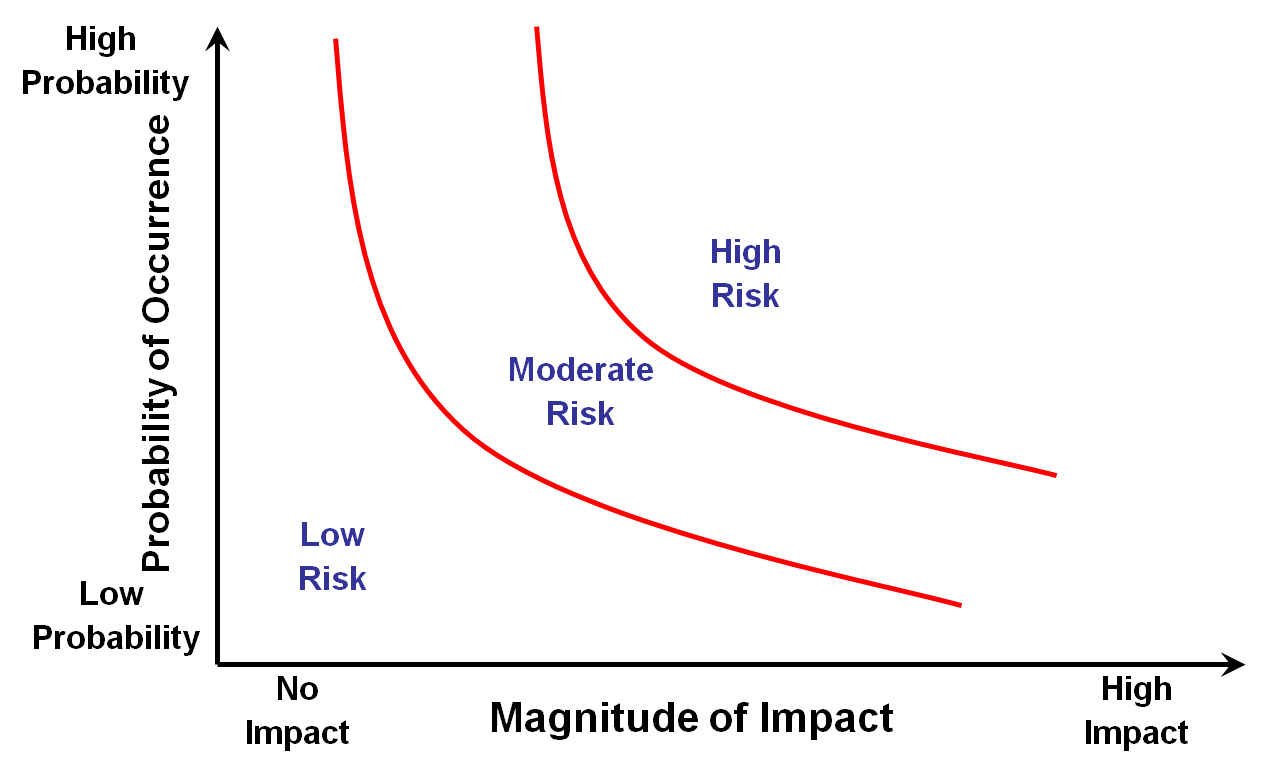
\includegraphics[width=10cm]{images/MagImpact.png}
	\label{fig:MagImpact}
\end{figure}


\end{frame}\begin{center}\line(1,0){250}\end{center}



\begin{frame}
\frametitle{Project Risk Management}
Risk is, in effect, a lack of knowledge of future events
\begin{itemize}
	\item Future events that are favourable are called opportunities
	\item Future events that are unfavourable are called risks
\end{itemize}
Another element of risk is its cause.
\begin{itemize}
	\item This can be something present or something missing
	\item This is referred to as a `hazard'
\end{itemize}
\end{frame}\begin{center}\line(1,0){250}\end{center}







\begin{frame}
\frametitle{Hazards}
Certain hazards can be overcome by:
\begin{itemize}
	\item Knowing what they are
	\item Taking action to overcome them
	\item So Risk is also a function of the hazard and the safeguard
\end{itemize}
Risk Increases with hazard and decreases with safeguard

\end{frame}\begin{center}\line(1,0){250}\end{center}





\begin{frame}
\frametitle{Tolerance for Risk}
	\begin{itemize}
		\item Depends on individuals and/or organisations.
		\item Some companies seek out risk, others avoid
	\end{itemize}
\begin{figure}[h]
	\centering
		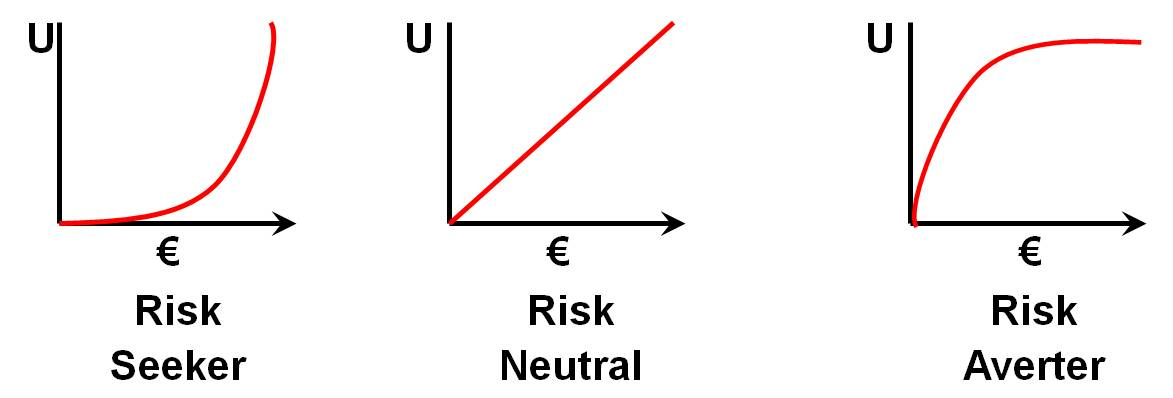
\includegraphics[width = 10cm]{images/Utility1.jpg}
	\label{fig:Utility1}
\end{figure}

\end{frame}\begin{center}\line(1,0){250}\end{center}





\begin{frame}
\frametitle{Project Risk Management}
Risk Seeker
\begin{itemize}
	\item PM's satisfaction increases at a greater rate as more money is at stake
\end{itemize}
Risk Averter
\begin{itemize}
	\item Utility rises at a decreasing rate.
\end{itemize}
As more money is at stake the project managers satisfaction diminishes
\end{frame}\begin{center}\line(1,0){250}\end{center}






\begin{frame}
\frametitle{Project Risk Management}
The objectives of Project Risk Management are 
\begin{itemize}
	\item to increase the probability and impact of positive events 
\item and to decrease the probability and impact of negative events
\end{itemize}
Project Risk Management includes:
\begin{itemize}
	\item Plan Risk Management
\item Identify Risks
\item Perform Qualitative Risk Analysis
\item Perform Quantitative Risk Analysis
\item Plan Risk Responses
\item Monitor and Control Risks
\end{itemize}
\end{frame}\begin{center}\line(1,0){250}\end{center}



\subsection{Plan Risk Mangement}


\begin{frame}
\frametitle{Plan Risk Management}
\begin{figure}
	\centering
		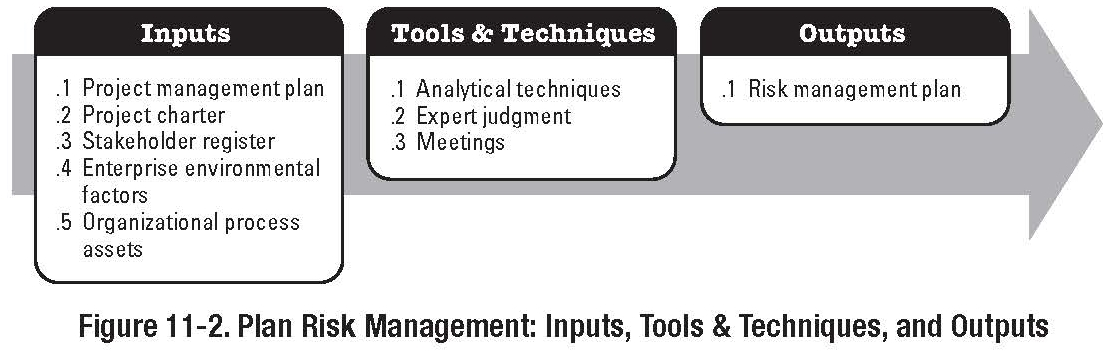
\includegraphics[width = 10cm]{images/Fig11-2.jpg}
	\label{fig:11-2}
\end{figure}
Part of the Planning Process Group
\end{frame}\begin{center}\line(1,0){250}\end{center}



\begin{frame}
\frametitle{Plan Risk Management}
Inputs
\begin{itemize}
	\item Enterprise Environmental Factors
\end{itemize}
Attitude towards risk and the risk tolerance of the organisation, and individuals
\begin{itemize}
	\item Organisational Process Assets
\end{itemize}
Predefined approaches to risk management, such as risk categories, standard templates, and authority levels for decision making
\begin{itemize}
	\item Project Scope Statement
	\item Cost/Schedule Management Plans
\end{itemize}
\end{frame}\begin{center}\line(1,0){250}\end{center}




\begin{frame}
\frametitle{Plan Risk Management}
Tools and Techniques
\begin{itemize}
	\item Planning Meetings and Analysis
	\item Meeting to develop Risk Management Plan
	\item Attendees may include PM, PM team, stakeholders
\end{itemize}
Outputs
\begin{itemize}
	\item Risk Management Plan
	\item Methodology
	\item Roles and Responsibilities
	\item Budgeting
	\item Timing
	\item Risk Categories
	\item Definitions of Risk Probability and Impact (Probability and Impact Matrix)
	\item Revised Stakeholders Tolerances
	\item Reporting Formats
	\item Tracking
\end{itemize}
\end{frame}\begin{center}\line(1,0){250}\end{center}





\begin{frame}
\frametitle{Risk Management Plan}

\begin{itemize}
	\item Methodology
	\item Defined approaches, tools, and data sources
		\begin{itemize}
			\item Roles and Responsibilities
		\end{itemize}
		\item Defines Lead, support and risk management team membership for each type of activity in the risk management plan, assigns people to these roles, and clarifies their responsibility
		\begin{itemize}
			\item Budgeting
		\end{itemize}
		\item Assigns resources and estimated costs needed for risk management.
		\begin{itemize}
			\item Included in the project baseline costs
		\end{itemize}
\end{itemize}
\end{frame}\begin{center}\line(1,0){250}\end{center}





\begin{frame}
\frametitle{Risk Management Plan}

\begin{itemize}
	\item Timing
	\begin{itemize}
		\item Defines when and how risk management processes will be performed
		\item Establishes Risk Management activities to be included in project schedule
	\end{itemize}
	\item Risk Categories
	\begin{itemize}
		\item Provides a structure that ensures a comprehensive, systematic process to identify risk.
		\item Risk Breakdown Structure (RBS)
	\end{itemize}
\end{itemize}
\end{frame}\begin{center}\line(1,0){250}\end{center}




\begin{frame}
\frametitle{Plan Risk Management}
\begin{figure}
	\centering
		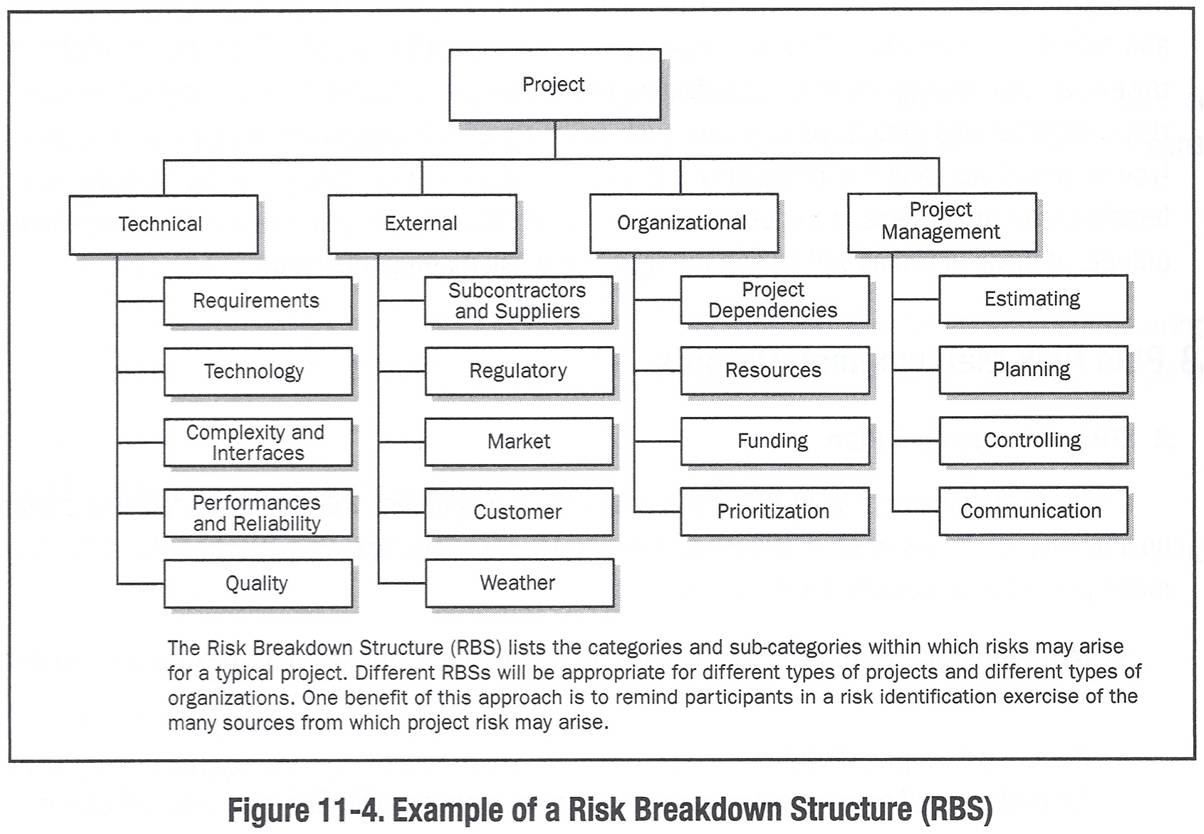
\includegraphics[width = 8cm]{images/RBS.jpg}
	\label{fig:11-4OLD}
\end{figure}
\begin{itemize}
\item Risk Breakdown Structure (RBS) From PMBOK 4
\end{itemize}
\end{frame}\begin{center}\line(1,0){250}\end{center}






\begin{frame}
\frametitle{Risk Management Plan}
Definitions of Risk Probability and Impact
\begin{itemize}
	\item The Quality and Credibility of the Qualitative Risk Analysis Process
	\item Assigns a relative scale for probability

	\begin{itemize}
		\item `very unlikely' to `almost certain'
		\item Very unlikely = Government not paying contractor
		\item Almost certain = Final account dispute
		\item May also be 1.0 to 0.0
	\end{itemize}
	\item Probability and Impact Matrix
\end{itemize}
\end{frame}\begin{center}\line(1,0){250}\end{center}






\begin{frame}
\frametitle{Plan Risk Management}
Impact Scale
\begin{figure}
	\centering
		\includegraphics[width = 9cm]{images/Table11-1.jpg}
	\label{tab:11-1}
\end{figure}
\end{frame}\begin{center}\line(1,0){250}\end{center}






\begin{frame}
\frametitle{Risk Management Plan}
Definitions of Risk Probability and Impact
\begin{itemize}
	\item Probability and Impact Matrix
\end{itemize}
\begin{figure}
	\centering
		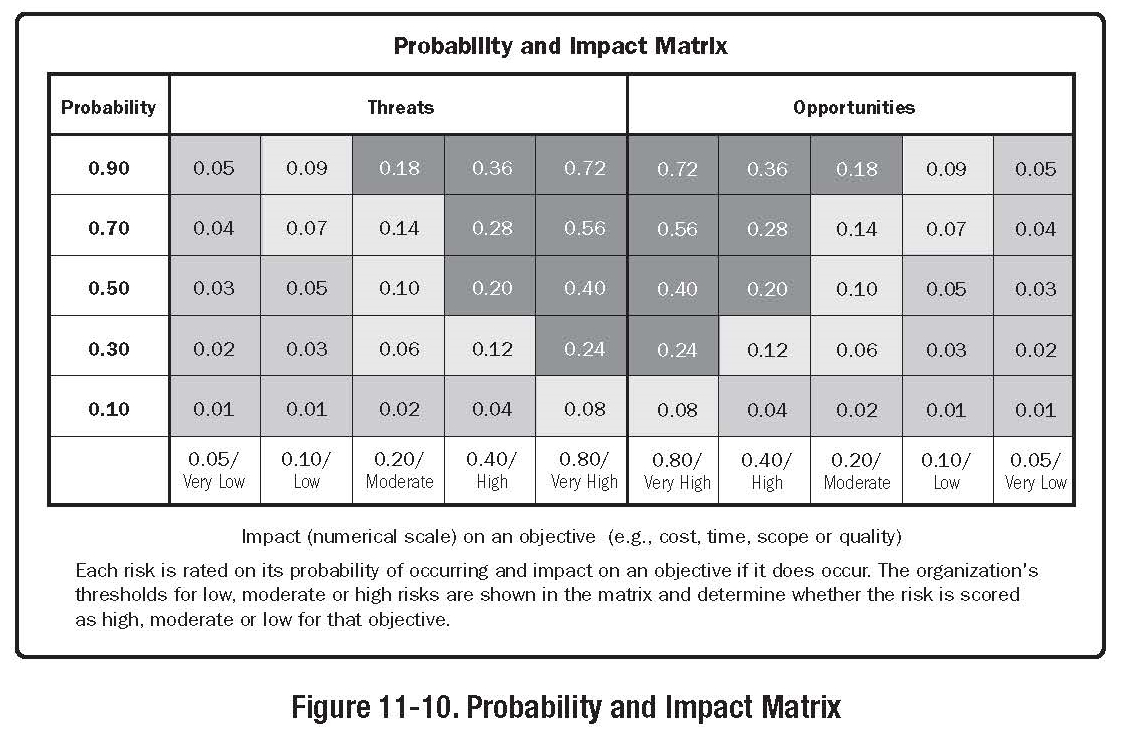
\includegraphics[width = 10cm]{images/Fig11-10.jpg}
	\label{fig:11-10}
\end{figure}
\end{frame}\begin{center}\line(1,0){250}\end{center}






\begin{frame}
\frametitle{Risk Management Plan}
Revised Stakeholders Tolerances - As project risks are identified, stakeholders may change their tolerance for specific risks.
\begin{itemize}
	\item Schedule Risks
	\item Budget Risk
	\item Quality Risk
\end{itemize}
Reporting Formats
\begin{itemize}
	\item Content and Format of Risk Register
	\item Defines how outcomes of risk management will be documented
\end{itemize}
Tracking
\begin{itemize}
	\item Documents how all facets of risk activities will be recorded for the benefit of the current project, future needs, and lessons learned
\end{itemize}
\end{frame}\begin{center}\line(1,0){250}\end{center}




\begin{frame}
\frametitle{Project Risk Management}
Because of the unique and temporary nature of projects, projects carry a greater level of risk than operations.\\

Risk may be defined as an uncertain event or condition that, if it occurs, has an effect on the project objectives.\\

\end{frame}\begin{center}\line(1,0){250}\end{center}






\begin{frame}
\frametitle{}
Managing project risk is an integral part of Project Management and critical to project success. 
Not managing project risk may result in:
\begin{itemize}
	\item Over Budget
	\item Over Time
	\item Poor Project Performance
	\item Loss of reputation
\end{itemize}
\end{frame}\begin{center}\line(1,0){250}\end{center}





\begin{frame}
\frametitle{Risk Management}

RM includes the processes concerned with identifying, analysis and responding to uncertainty.\\
The purpose of risk management is to identify the risk factors for a project and then establish a risk management plan to minimize the probability \& impact that the negative risk event will have on the project. \\
The goal of risk management is to identify project risks and develop strategies, which either significantly reduce them or take steps to avoid them altogether.\\

\end{frame}\begin{center}\line(1,0){250}\end{center}






\begin{frame}
\frametitle{Risk Management}
A Risk is a potential future problem that has not yet occurred 
\begin{itemize}
	\item A reactive project manager tries to resolve issues when they occur. 
\item A proactive project manager tries to resolve potential problems before they occur. 
\end{itemize}
\end{frame}\begin{center}\line(1,0){250}\end{center}





\begin{frame}
\frametitle{Risk Management}
\begin{itemize}
\item No universal definition of the terms used. 
\item The scope and quality knowledge areas need review to see opportunities or threats. 
\item A single risk event may have multiple effects. 
\item Opportunities for one stakeholder may be a threat for another. 
\item Mathematical techniques used may create a false impression of precision and reliability.
\item Risk probability x Risk value (their product) is a typical risk quantification procedure. 
\item Responses include: contracting, bonding, contingency planning, insurance, alternative strategies. 
\end{itemize}
\end{frame}\begin{center}\line(1,0){250}\end{center}





\begin{frame}
\frametitle{Risk Management}
\begin{itemize}
\item RM includes the processes concerned with identifying, analysis and responding to uncertainty. 
\item The key principle of Risk Management is to foresee problems before they occur and plan responses to them
\item Risk may be defined as an uncertain event or condition that, if it occurs, has an effect on the project objectives.
\end{itemize}
\end{frame}\begin{center}\line(1,0){250}\end{center}


\begin{frame}
\frametitle{Risk Management}
RM includes the processes concerned with identifying, analysis and responding to uncertainty. 
\begin{itemize}
	\item Risk Identification
	\item Risk Quantification
	\item Risk Response Development 
	\item Risk Response Control \& Monitoring
\end{itemize}

\end{frame}\begin{center}\line(1,0){250}\end{center}






\begin{frame}
\frametitle{Risk Management}
IDENTIFICATION: 
\begin{itemize}
	\item Sources, events, probability x amount at stake
\end{itemize}
QUANTIFICATION:  
\begin{itemize}
	\item Influence diagrams, probability distribution, probability trees, risk modelling, sensitivity profiles
\end{itemize}
RESPONSE DEVELOPMENT: 
\begin{itemize}
	\item Avoid, transfer, mitigate, retain/accept, 
\end{itemize}
RESPONSE CONTROL: 
\begin{itemize}
	\item Execute plan in event 
\end{itemize}
\end{frame}\begin{center}\line(1,0){250}\end{center}



\subsection{Risk Analysis}


\begin{frame}
\frametitle{Risk Analysis}
Risk needs to be measured in terms of its potential impact or cost on the project, and the probability that the risk event will actually occur.  
\end{frame}\begin{center}\line(1,0){250}\end{center}




\begin{frame}
\frametitle{Qualitative Analysis}
\begin{itemize}
\item The overall risk measure against each risk is a combination of both of the probability that it will occur and the impact that the risk would have should it occur.  
\item Both the probability and impact are qualitative measures based on the team experience and technical knowledge. 
\item Risk Prioritisation
\begin{itemize}
	\item The risks analysed are prioritised for action
\end{itemize}
\end{itemize}
\end{frame}\begin{center}\line(1,0){250}\end{center}






\begin{frame}
\frametitle{Risk Response}
For each risk identified a Risk Response Strategy that should be considered. Choices are:
\begin{itemize}
	\item Risk Avoidance
	\item Risk Transference
	\item Risk Reduction
	\item Risk Acceptance
\end{itemize}
\end{frame}\begin{center}\line(1,0){250}\end{center}






\begin{frame}
\frametitle{Risk Levels}
\begin{itemize}
	\item Risk occurs in different ways at every level of an organisation.
	\item Risk may occur at the strategic level, programme level, project level and operational level.
	\item Strategic Risk may be described as risk to the business strategy and is the concern and responsibility of the Management team.
\end{itemize}
\end{frame}\begin{center}\line(1,0){250}\end{center}






\begin{frame}
\frametitle{Risk Levels - Programme Risk}
Risk at this level could be due to:
\begin{itemize}
	\item Interdependencies between projects
	\item Overall resource levels
	\item Changes in approved budget
	\item Materials supply capability
	\item The wider system - the political, economic, social, technological environment
\end{itemize}
These risks affect many projects simultaneously, and are managed by the Programme manager.
\end{frame}\begin{center}\line(1,0){250}\end{center}






\begin{frame}
\frametitle{Risk Levels - Project \& Operational}
Project Risks:  
	\begin{itemize}
		\item Risks at this level are threats to the success of a single project, and most often impact the principal targets of scope, time, cost, and quality, though may impact other knowledge areas at the same time. Risks that threaten the success of the project are the responsibility of the Project manager.
	\end{itemize}
Operational Risk: 
	\begin{itemize}
		\item The day-to-day operations are also subject to risks. Matters such as health and safety, industrial relations are amongst the operational risks faced by an organisation.
	\end{itemize}
The identification of risks at different organisational levels allow identification of who has responsibility for the risk.

\end{frame}\begin{center}\line(1,0){250}\end{center}






\begin{frame}
\frametitle{Risk and the Project Life Cycle}
\begin{itemize}
\item The project life cycle which establishes the phases through which a project will pass is so designed to enable the management of risk. 
\item The Knowledge areas also enable the effective management of projects. 
\item The process of risk management requires that risk be managed continuously throughout the life of the project.
\end{itemize}
\end{frame}\begin{center}\line(1,0){250}\end{center}





\begin{frame}
\frametitle{Risk Identification}
\begin{itemize}
\item The identification of risk should occur as early as possible - i.e. in the conception and definition phase. Risk identification requires an understanding of the project scope and objectives and deciding what may prevent the achievement of them.
\item The project charter will set out the high level risks to the project. It will also identify the success criteria by which the project will be judged later.
\begin{itemize}
	\item The potential risks to the project are identified as comprehensively as possible
\item Can be helpful to brainstorm in groups and draw on the experience of the project participants
\end{itemize}
\end{itemize}
\end{frame}\begin{center}\line(1,0){250}\end{center}






\begin{frame}
\frametitle{Risk Identification}
\begin{itemize}
\item The feasibility study, if required, will identify and assess the risks in determining the best way of undertaking the project and to determine if proceeding with the project is the best option.
\item In the planning phase the project manager in the development of the project plan will evaluate the project risk and develop a risk response plan.
\item As part of implementation these plans will be executed. The process of risk identification and analysis should be re-applied through the implementation phase of the project to re-evaluate project risks
\end{itemize}
\end{frame}\begin{center}\line(1,0){250}\end{center}






\begin{frame}
\frametitle{Risk Categories}
Technical Risks
\begin{itemize}
	\item Robustness of the solution
	\item Complexity of the system
	\item Ownership
\end{itemize}
Business / Management Risk
\begin{itemize}
	\item Financing
	\item Revenue / Cost / Margin
	\item Shareholders
\end{itemize}
\end{frame}\begin{center}\line(1,0){250}\end{center}


\begin{frame}
\frametitle{Risk Categories}
Delivery / Operational Risks
\begin{itemize}
	\item Training \& Training Support
	\item Human Resource Considerations
	\item Complexity
	\item Product Life Cycle
	\item On going support
\end{itemize}
Cost
Schedule
\end{frame}\begin{center}\line(1,0){250}\end{center}



\begin{frame}
\frametitle{Risk Recording and Scoring}
A table for recording project risks is called a Risk Log. 
		\begin{itemize}
			\item All identified risks must be recorded in the Risk Log. Risks with a significant potential impact may cause immediate alteration of the Project Plan, and therefore another iteration of risk identification is required
		\end{itemize}

Risk Analysis
	\begin{itemize}
		\item Risk analysis involves assessing the probability of a risk occurring and its likely impact if it does occur. The ranking or scoring of risk involves the following calculation
	\end{itemize}
Risk Ranking/Scoring = Probability x Impact
	\begin{itemize}
		\item (High, medium , low)
	\end{itemize}
\end{frame}\begin{center}\line(1,0){250}\end{center}




\begin{frame}
\frametitle{}
\begin{figure}[h]
	\centering
		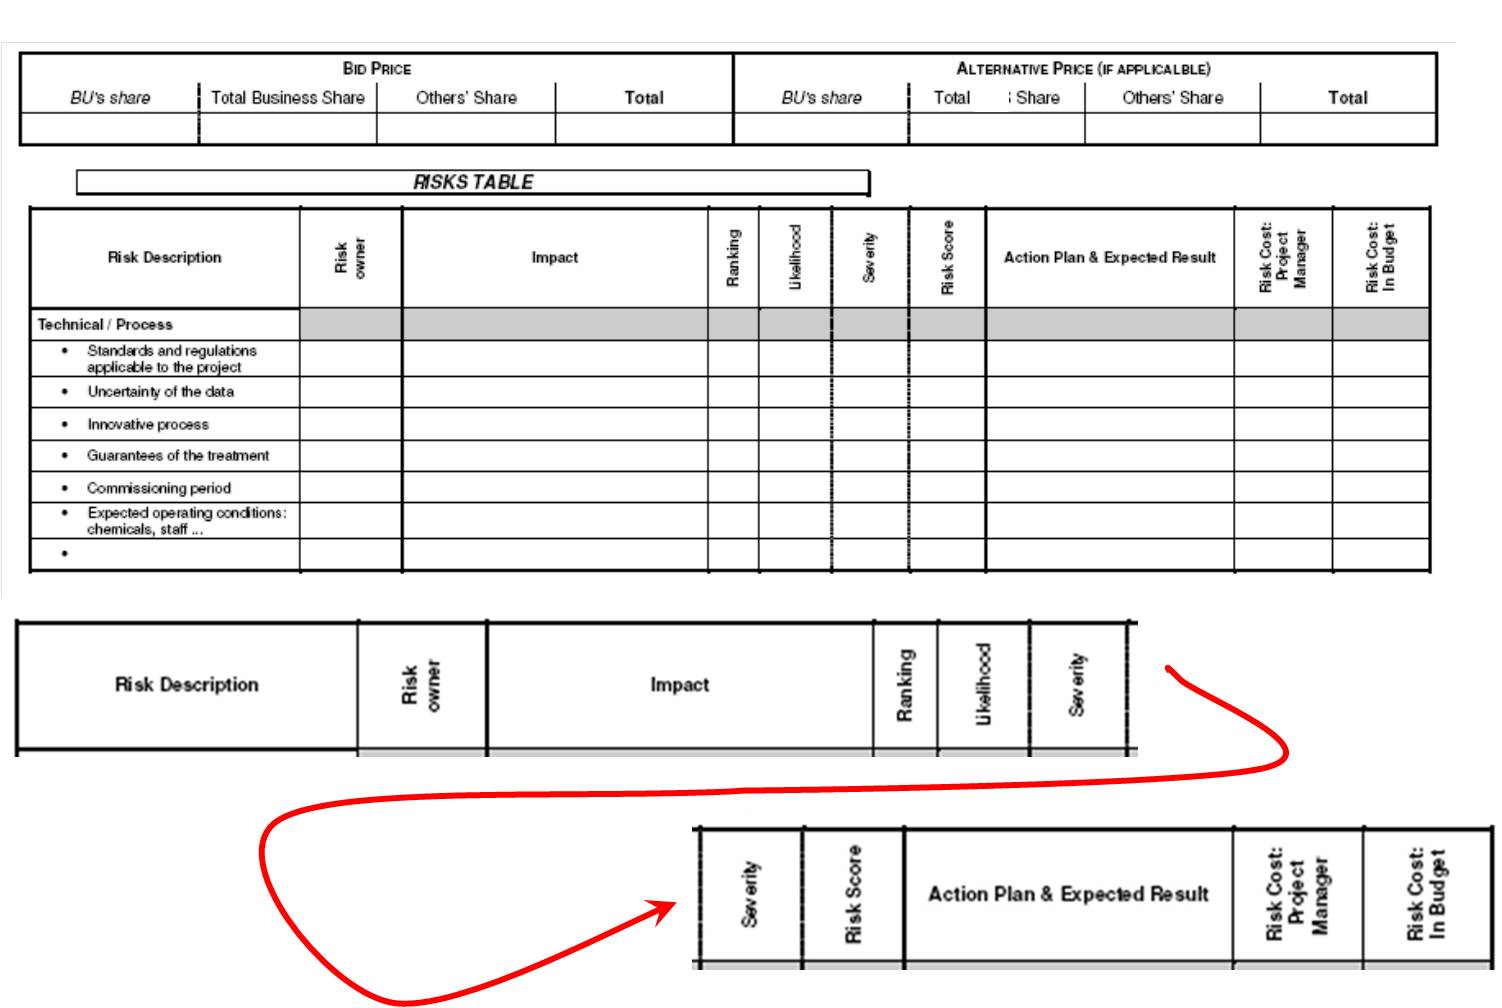
\includegraphics[width = 10 cm]{images/veo1.jpg}
	\label{fig:veo1}
\end{figure}

\end{frame}\begin{center}\line(1,0){250}\end{center}




\begin{frame}
\frametitle{}
\begin{figure}
	\centering
		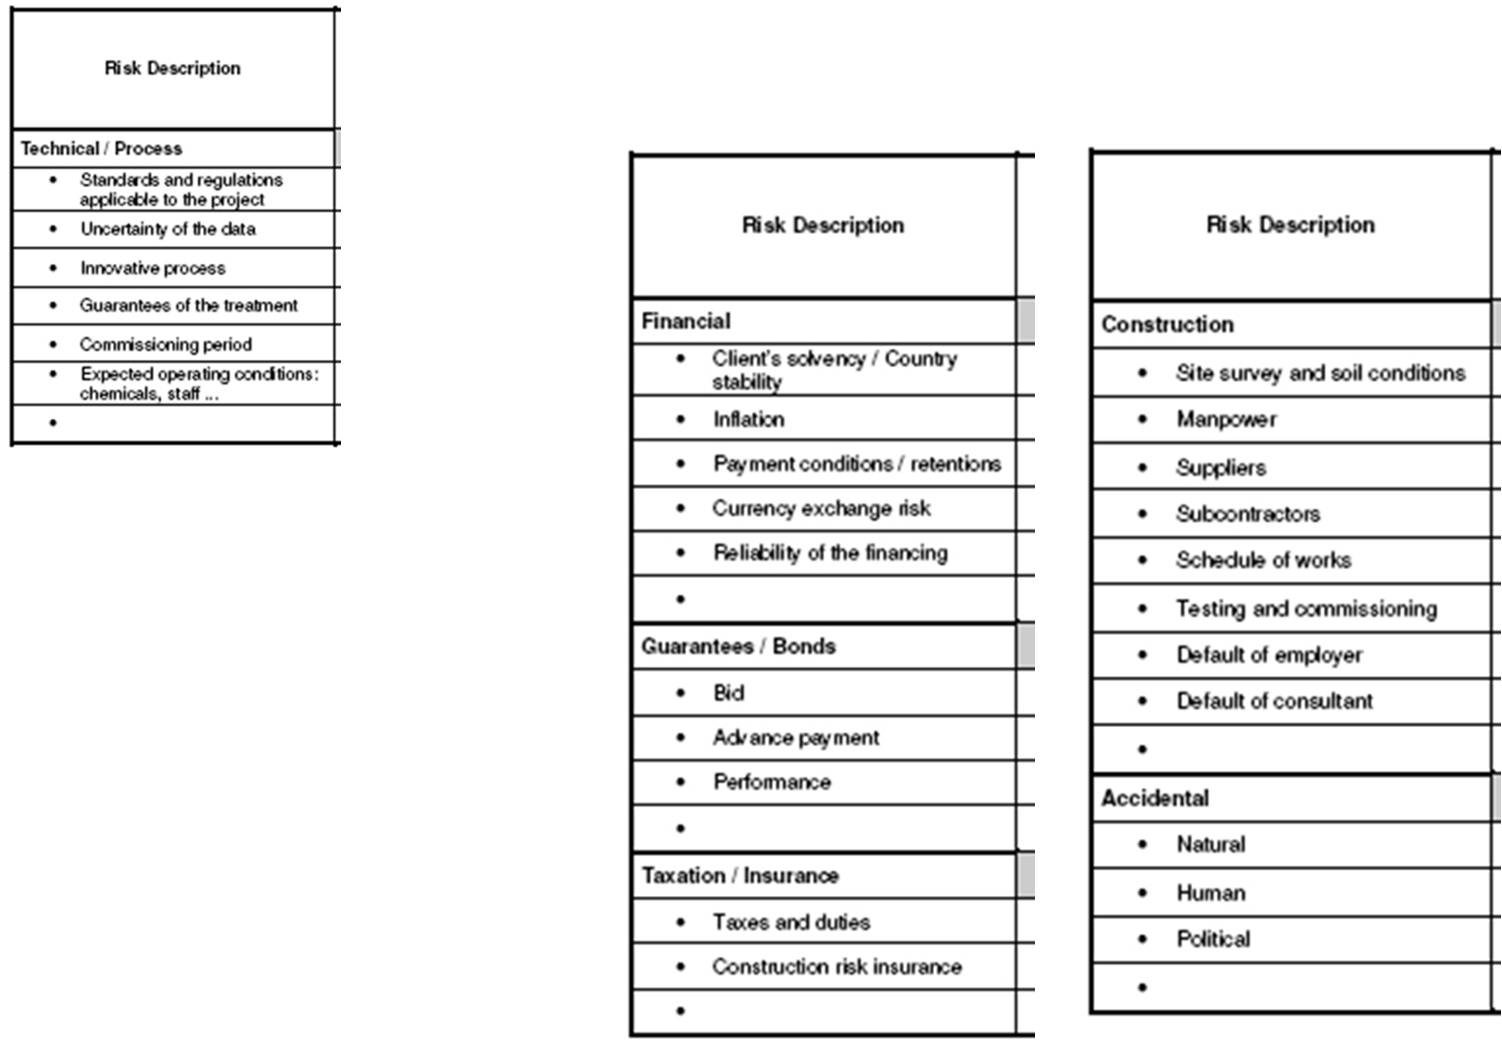
\includegraphics[width = 8 cm]{images/veo2.jpg}
	\label{fig:veo2}
\end{figure}


\end{frame}\begin{center}\line(1,0){250}\end{center}




\begin{frame}
\frametitle{}
\begin{figure}
	\centering
		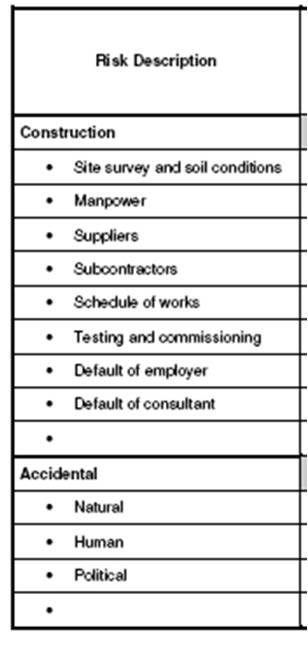
\includegraphics[width = 3 cm]{images/veo3.jpg}
	\label{fig:veo3}
\end{figure}

\end{frame}\begin{center}\line(1,0){250}\end{center}




\begin{frame}
\frametitle{Qualitative Analysis}
\begin{figure}
	\centering
		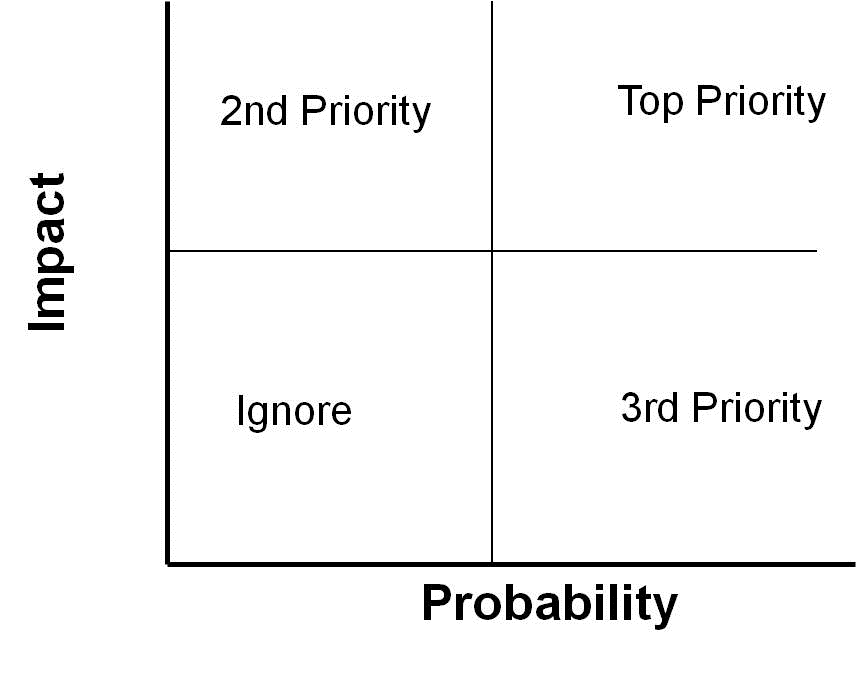
\includegraphics[width = 5cm ]{images/Matrix3.jpg}
	\label{fig:Matrix3.png}
\end{figure}

\end{frame}\begin{center}\line(1,0){250}\end{center}




\begin{frame}
\frametitle{Risk Importance}
\begin{itemize}
\item Consider the relative impact each risk will have on the project if it happens. 
\item Note that low probability risks are often high on impact 
\item Alternatively the Risk Probability/Impact Matrix maybe used to establish risk ranking by placing each risk in its correct box in the grid.
\item The distribution of risks over this matrix gives an overall view of the project risk level. 
\begin{itemize}
	\item Low-Medium-High
\end{itemize}
\end{itemize}
\end{frame}\begin{center}\line(1,0){250}\end{center}





\begin{frame}
\frametitle{Risk Probability \& Impact Matrix}
\begin{figure}
	\centering
		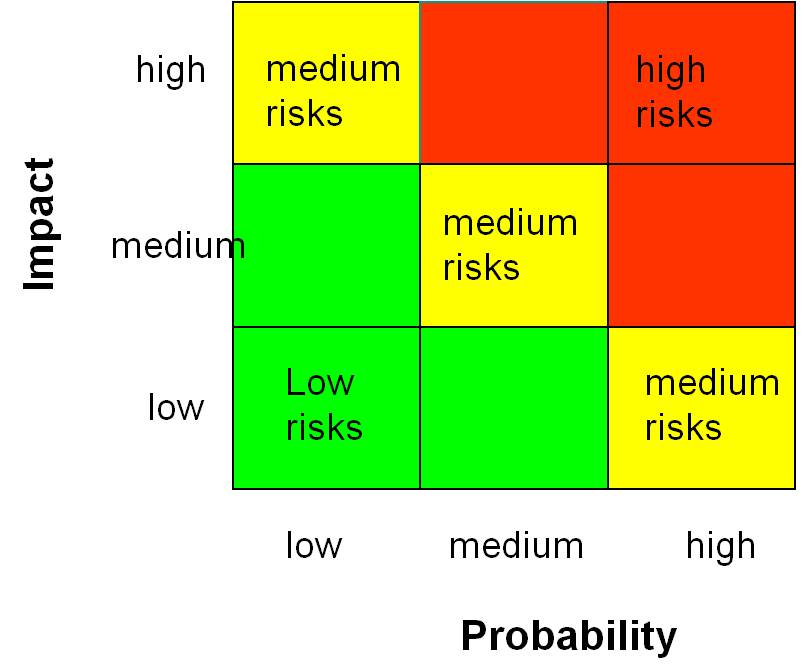
\includegraphics[width = 5cm]{images/Matrix2.jpg}
	\label{fig:Matrix2}
\end{figure}

\end{frame}\begin{center}\line(1,0){250}\end{center}





\begin{frame}
\frametitle{Risk Response}
Once the risks are identified, analysed and prioritised, a plan of action to manage them is developed. \\
There are 5 response types. (PMBOK gives 4) These are
\begin{itemize}
	\item Avoidance, 
\item Transfer, 
\item Reduction, 
\item Contingency  
\item Acceptance. 
\end{itemize}
If a risk has more than one response option, put multiple entries in the Risk Register

\end{frame}\begin{center}\line(1,0){250}\end{center}




\begin{frame}
\frametitle{Risk Response}
\begin{figure}
	\centering
		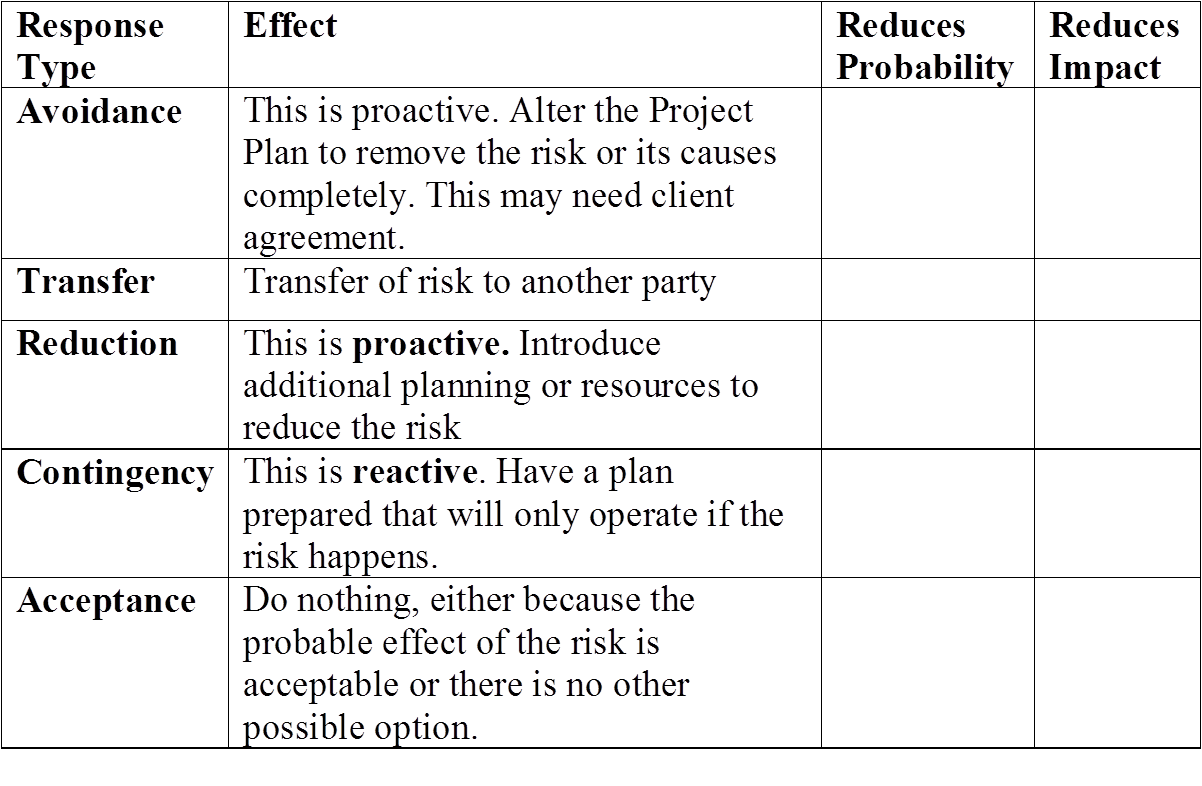
\includegraphics[width = 10cm ]{images/Matrix.png}
	\label{fig:Matrix}
\end{figure}

\end{frame}\begin{center}\line(1,0){250}\end{center}





\begin{frame}
\frametitle{Response Selection}
\begin{itemize}
\item Do not dwell too long on the Response Type - it is more important to record the details of your risk mitigation.
\item Responses should be consistent with the project priorities. For example if the schedule is the top priority, try not to plan responses that will add time to schedule.
\item Make certain that the response you plan does not end up costing more time or money that the risk you are tying to cover. 
\item As you plan each response, identify who is responsible.
\item The same risk occurring at different times may require a different response. Note these as separate entries in the Risk Log.
\item Given your planned risk responses, reassess the probability and impact ratings for each risk. The aim is reduce each Risk Rating, and therefore the overall project risk.
\end{itemize}
\end{frame}\begin{center}\line(1,0){250}\end{center}





\begin{frame}
\frametitle{Risk Monitoring}
\begin{itemize}
\item Risks change over time. Having created the Risk Log during the Planning stage, these risks are monitored and controlled during the project execution. 
\item Update the Risk Log as old risks diminish and new risks appear. Reappraise the risk responses in the light of experience and progress. For a long project, this should be done at least monthly.
\item Sort the Risk Log in order of reducing rank. Review and monitor risks in order of priority
\end{itemize}
\end{frame}\begin{center}\line(1,0){250}\end{center}





\begin{frame}
\frametitle{Risk Reporting}
\begin{itemize}
\item There may be examples of single, high-ranking project risks that have such a significant impact on the project; they need to be reported singly to the Programme Management Office as required. 
\item This would include risks that would:
\begin{itemize}
	\item Completely halt or unacceptably delay the project or
\item Cause over expenditure for the project,
\item Create a breech of legislation or law, such as Health \& Safety Legislation etc.
\item Make the planned scope impossible to deliver
\end{itemize}
\end{itemize}
\end{frame}\begin{center}\line(1,0){250}\end{center}




\begin{frame}
\frametitle{Decision Trees}
\begin{itemize}
\item Decision trees are composed of nodes(circles, squares and triangles) and branches(lines).
\item The nodes represent points in time. A decision node(a square) is a time when the decision maker makes a decision. A probability node(a circle) is a time when the result of an uncertain event becomes known. An end node(a triangle) indicates that the problem is completed -all decisions have been made, all uncertainty have been resolved and all payoffs have been incurred.
\end{itemize}
\end{frame}\begin{center}\line(1,0){250}\end{center}







\begin{frame}
\frametitle{Decision Trees}
\begin{itemize}
\item Time proceeds from left to right. This means that branches leading into a node (from the left) have already occurred. Any branches leading out of a node (to the right) have not yet occurred.
\item Branches leading out of a decision node represent the possible decisions; the decision maker can choose the preferred branch. Branches leading out of probability nodes represent the possible outcomes of uncertain events; the decision maker has no control over which of these will occur.
\end{itemize}
\end{frame}\begin{center}\line(1,0){250}\end{center}



\begin{frame}
\frametitle{Decision Trees}
\begin{itemize}
\item Probabilities are listed on probability branches. These probabilities are conditional on the events that have already been observed (those to the left). Also, the probabilities on branches leading out of any particular probability node must sum to 1.
\item Individual monetary values are shown on the branches where they occur, and cumulative monetary values are shown to the right of the end nodes. (Two values are often found to the right of each node: the top one is the probability of getting to that end node, and the bottom one is the associated monetary value).
\end{itemize}
\end{frame}\begin{center}\line(1,0){250}\end{center}









\begin{frame}
\frametitle{Decision Making}
Decision Making Processes: 
\begin{itemize}
\item collect information
\item establish root cause
\item generate solutions
\item select best option
\item implement/monitor
\end{itemize}
\end{frame}\begin{center}\line(1,0){250}\end{center}





\begin{frame}
\frametitle{Decision Trees}
\begin{figure}
	\centering
		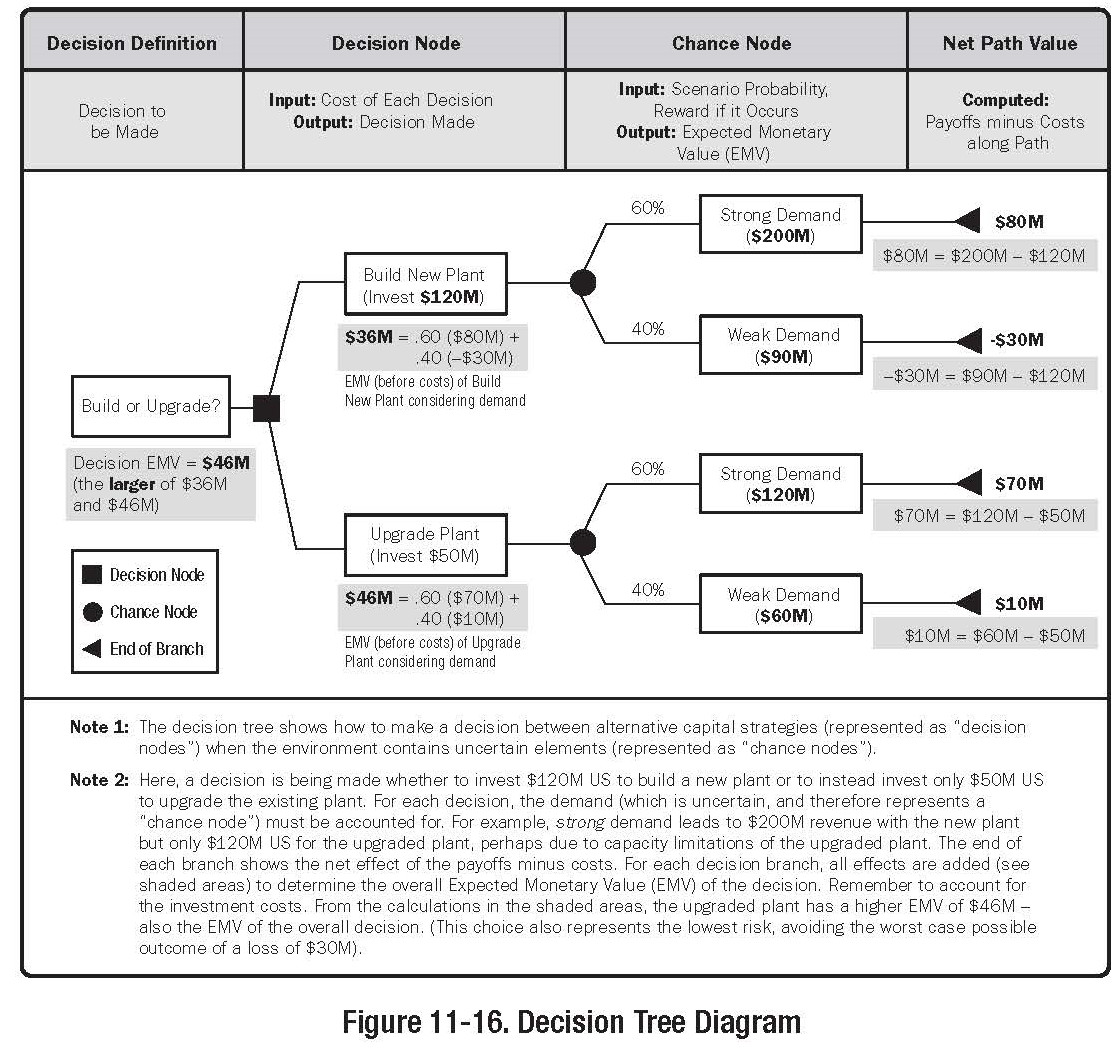
\includegraphics[width = 7cm]{images/Fig11-16.jpg}
	\label{fig:11-16}
\end{figure}
\end{frame}\begin{center}\line(1,0){250}\end{center}






\begin{frame}
\frametitle{}
\begin{figure}
	\centering
		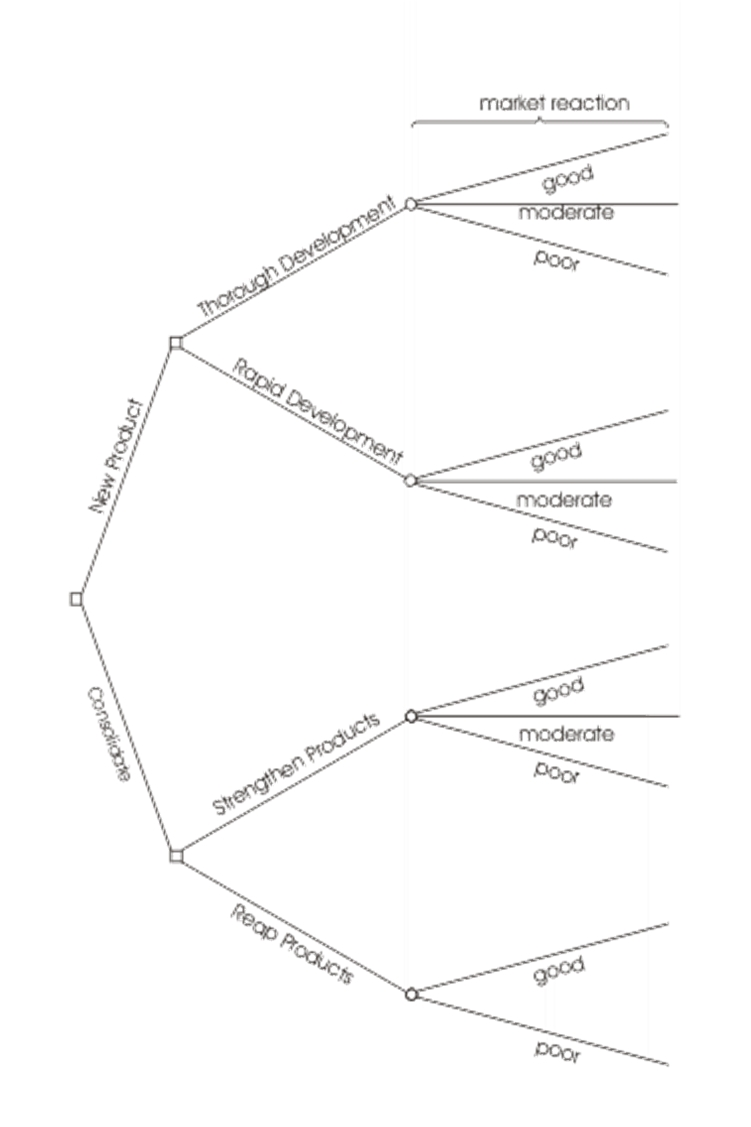
\includegraphics[width = 5cm]{images/evmtree2.jpg}
	\label{fig:tree1}
\end{figure}
\end{frame}\begin{center}\line(1,0){250}\end{center}






\begin{frame}
\frametitle{}
\begin{figure}
	\centering
		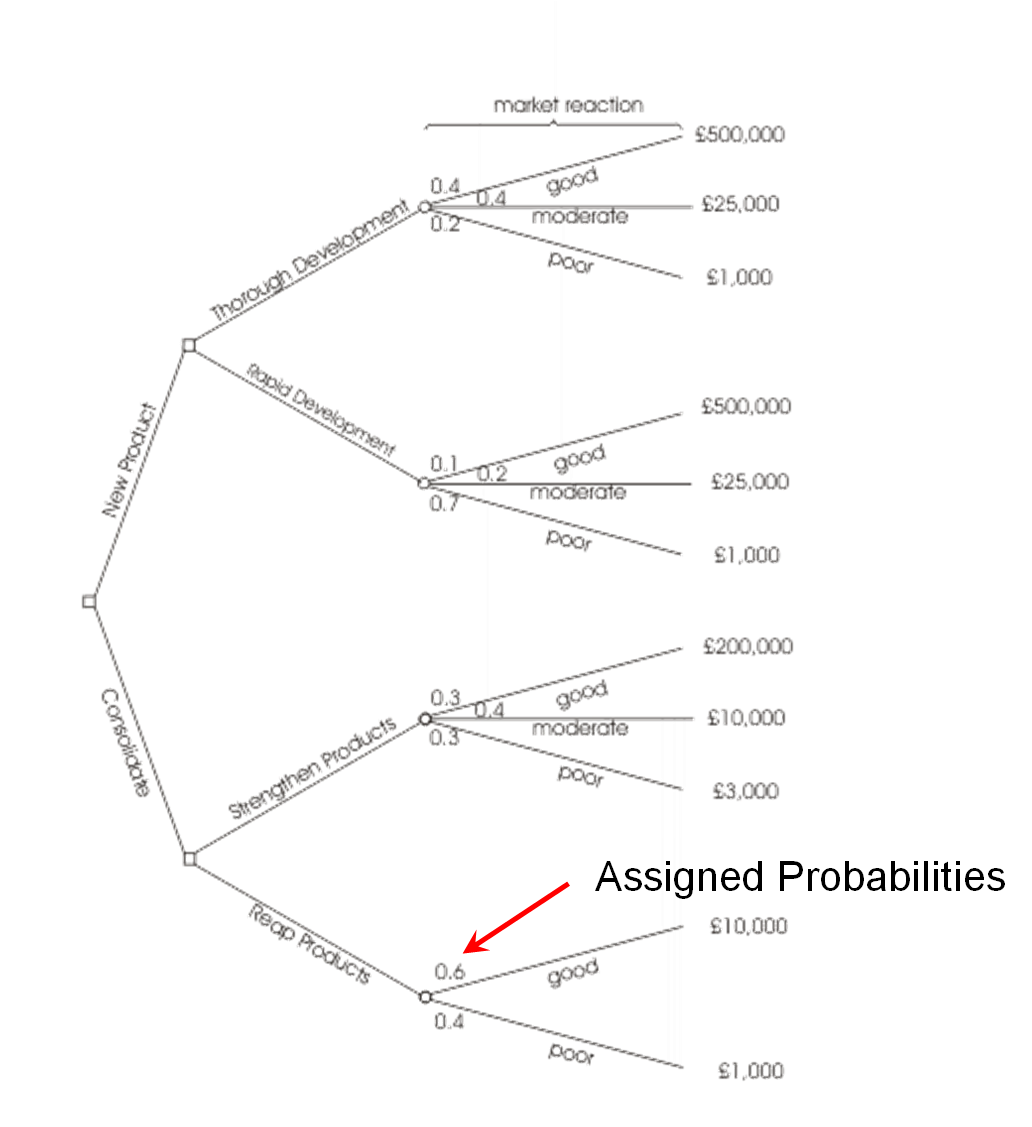
\includegraphics[width = 6cm]{images/evmtree1.jpg}
	\label{fig:tree2}
\end{figure}
\end{frame}\begin{center}\line(1,0){250}\end{center}






\begin{frame}
\frametitle{}
\begin{figure}
	\centering
		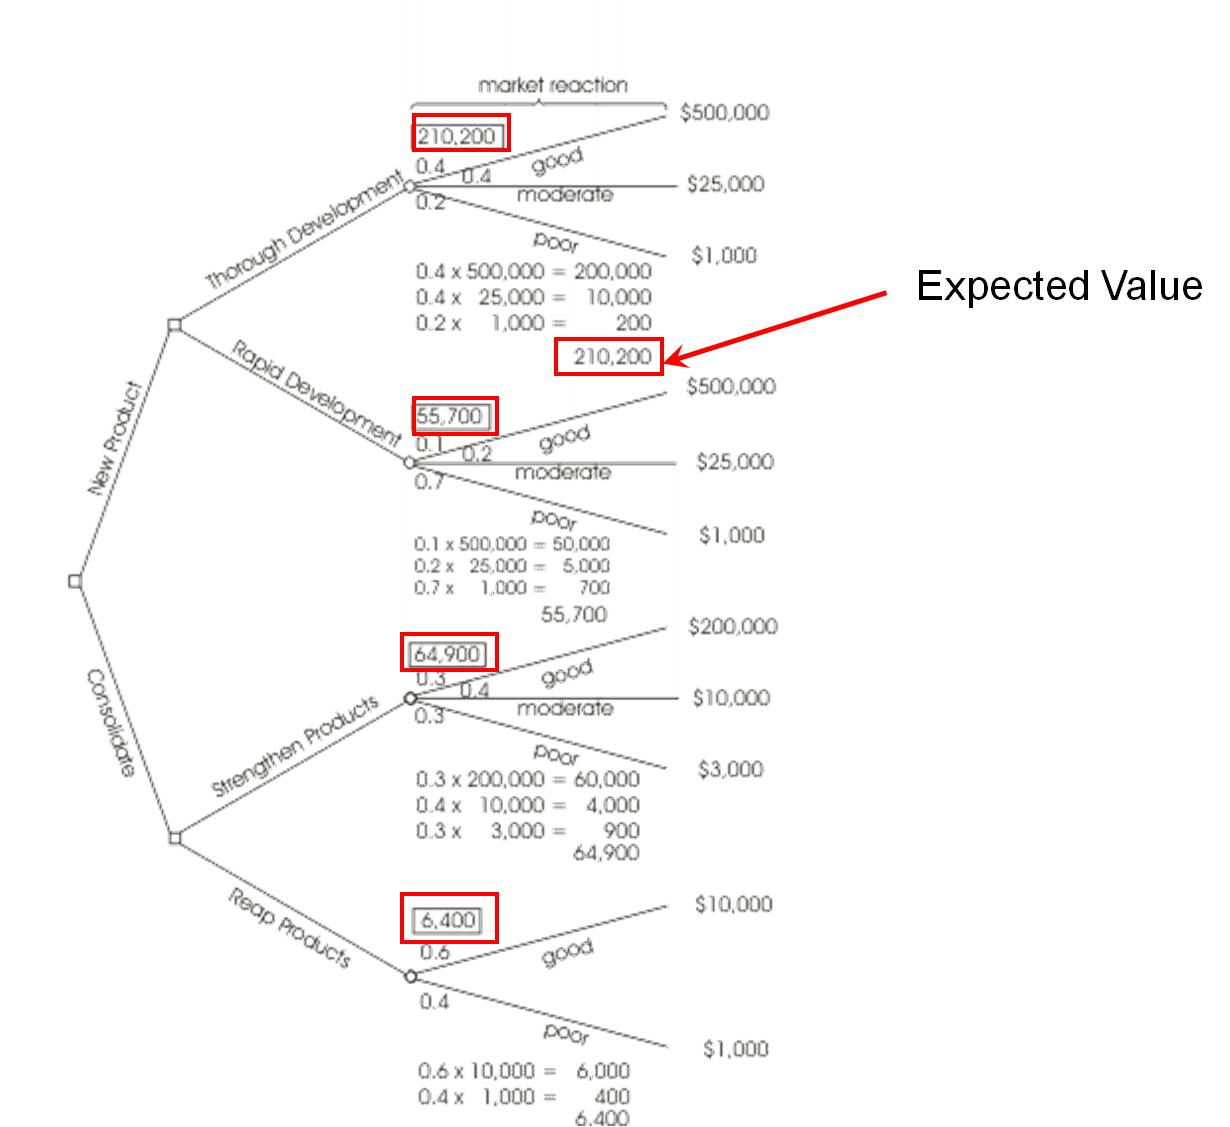
\includegraphics[width = 7cm]{images/evmtree.jpg}
	\label{fig:tree3}
\end{figure}
\end{frame}\begin{center}\line(1,0){250}\end{center}







\begin{frame}
\frametitle{Tree Construction}
\begin{itemize}
	\item Identify the decision points and alternatives actions available at each point
	\item Identify the uncertainties
	\item Estimate quantitative information (costs of possible outcomes, gains resulting from outcomes, probabilities of chance events)
	\item Define criteria of desirability
	\item Evaluate tree
\end{itemize}
\end{frame}\begin{center}\line(1,0){250}\end{center}






\begin{frame}
\frametitle{Key Points}
Decision trees provide an effective method of Decision Making because they:
\begin{itemize}
	\item Clearly lay out the problem so that all options can be challenged 
	\item Allow us to analyze fully the possible consequences of a decision 
	\item Provide a framework to quantify the values of outcomes and the probabilities of achieving them 
	\item Help us to make the best decisions on the basis of existing information and best guesses. 
\end{itemize}
\end{frame}\begin{center}\line(1,0){250}\end{center}







\begin{frame}
\frametitle{Need for Care}
\begin{itemize}
\item As with all Decision Making methods, decision tree analysis should be used in conjunction with common sense - decision trees are just one important part of your Decision Making tool kit. 
\end{itemize}
\end{frame}\begin{center}\line(1,0){250}\end{center}






\begin{frame}
\frametitle{Quantitative Risk Analysis}
\begin{figure}
	\centering
		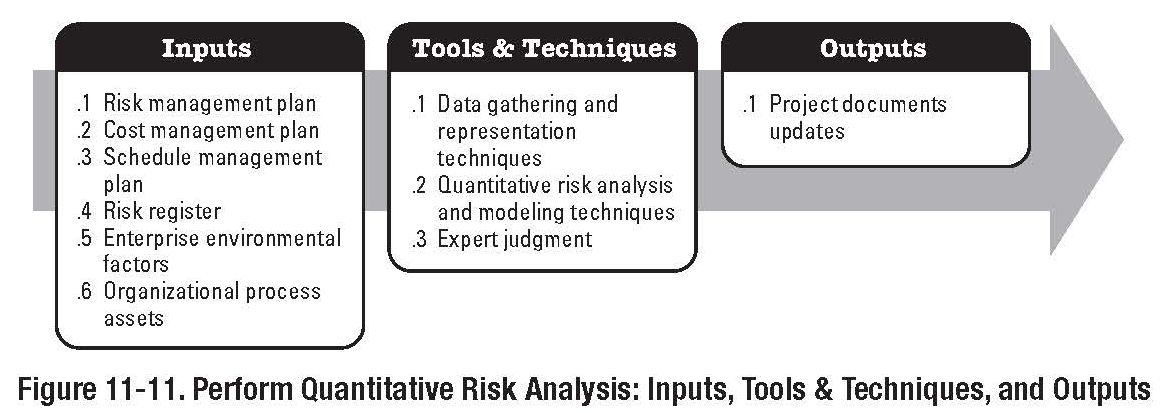
\includegraphics[width = 10cm]{images/Fig11-11.jpg}
	\label{fig:11-11}
\end{figure}
Part of the Planning Process Group
\end{frame}\begin{center}\line(1,0){250}\end{center}






\begin{frame}
\frametitle{Quantitative Risk Analysis}
\begin{itemize}
	\item Quantitative Risk Analysis is performed on Risks that have been prioritised by the Qualitative Risk Analysis Process
	\item The Quantitative Risk Analysis process is designed to
	\begin{itemize}
		\item Quantify the possible outcomes for the project and their probability 
		\item Assess the probability of achieving specific project goals
		\item Identify risks requiring the most attention by quantifying their relative contribution to the overall project risks
		\item Identify realistic and achievable cost, schedule, or scope targets, given the project risks
		\item Determine the best PM decisions when conditions or outcomes are uncertain 
	\end{itemize}
\end{itemize}
\end{frame}\begin{center}\line(1,0){250}\end{center}






\begin{frame}
\frametitle{Quantitative Risk Analysis}
\begin{itemize}
\item Inputs
\begin{itemize}
	\item Risk Register
\end{itemize}
\item List of identified risks, relative priority and ranking, etc.
\begin{itemize}
	\item Risk Management Plan
\end{itemize}
\item Roles and Responsibilities, Budgets, Schedules, etc.
\begin{itemize}
	\item Project Schedule Management Plan
\item Project Cost Management Plan
\item Organisational Process Assets
\end{itemize}
\item Information on prior, similar projects
\item Studies of similar projects
\item Risk Databases
\end{itemize}
\end{frame}\begin{center}\line(1,0){250}\end{center}







\begin{frame}
\frametitle{Quantitative Risk Analysis}
\begin{itemize}
	\item Tools and Techniques
		\begin{itemize}
			\item Data Gathering and Representation Techniques
		\end{itemize}
	\item Interviewing
		\begin{itemize}
			\item Used to quantify the probability and impact of risks on project objectives
		\end{itemize}
	\item Breakdown into `optimistic', `most-likely', and `pessimistic' 
	\item three point estimates
	\item Can provide information on the reliability and credibility of the analysis
	\item Probability Distributions
		\begin{itemize}
			\item Not all probabilities are normally distributed.
			\item For our work, we will only consider the normally distributed probabilities (PERT)
		\end{itemize}
	\item Expert Judgement
		\begin{itemize}
			\item Internal or External Experts
		\end{itemize}
\end{itemize}
\end{frame}\begin{center}\line(1,0){250}\end{center}





%	\begin{frame}
%	\frametitle{Quantitative Risk Analysis}
%	Interviewing
%	\begin{figure}
%		\centering
%			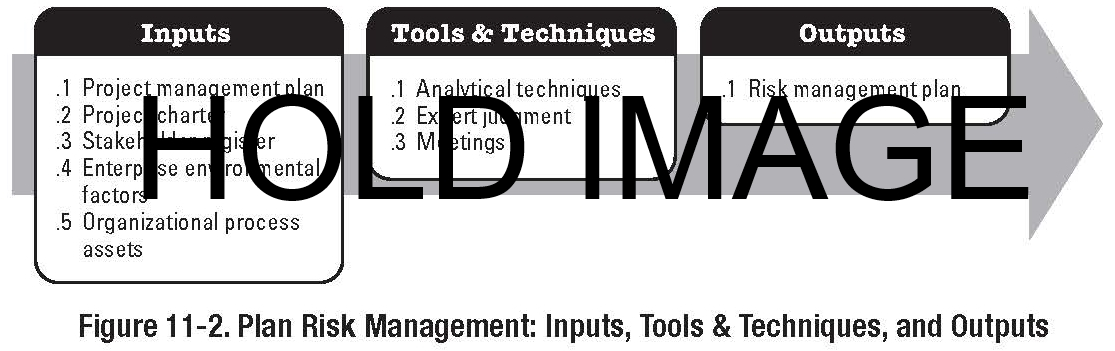
\includegraphics[width = 10cm]{images/MilFoot.jpg}
%		\label{fig:11-13}
%	\end{figure}
%	\end{frame}\begin{center}\line(1,0){250}\end{center}
	
	
	
%	\begin{frame}
%	\frametitle{Quantitative Risk Analysis)
%	Probability Distributions
%	\begin{figure}
%		\centering
%			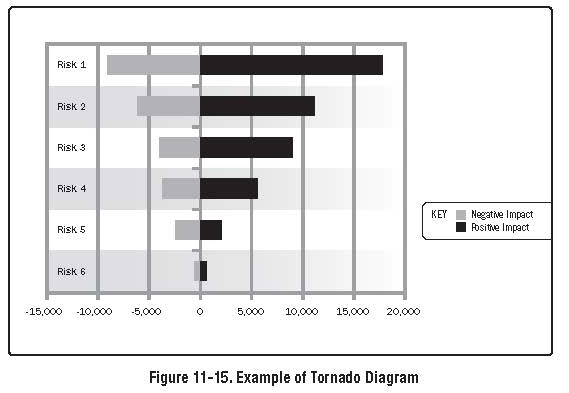
\includegraphics{images/Fig11-15.jpg}
%		\label{fig:Fig11-14}
%	\end{figure}
%	\end{frame}\begin{center}\line(1,0){250}\end{center}






\begin{frame}
\frametitle{Quantitative Risk Analysis}
\begin{itemize}
	\item Tools and Techniques
	\begin{itemize}
		\item Quantitative Risk Analysis and Modelling Techniques
	\end{itemize}
	\item Sensitivity Analysis
	\begin{itemize}
		\item Helps to determine which risks have the most potential impact on the project
		\item Examines the extent to which an individual project element will affect the project, when all other uncertain elements are held at `baseline'.
	\end{itemize}
	\item Expected Monetary Value Analysis
	\begin{itemize}
		\item EVM is a statistical concept that calculates the average outcome when the future includes scenarios that may or may not happen.
		\item EVM is calculated by multiplying each possible outcome by its probability
		\item Used in Decision Tree Analysis
	\end{itemize}
	\item Decision Tree Analysis
	\item Modelling and Simulation
\end{itemize}
\end{frame}\begin{center}\line(1,0){250}\end{center}






\begin{frame}
\frametitle{Quantitative Risk Analysis}
\begin{itemize}
\item Tools and Techniques
\begin{itemize}
	\item Quantitative Risk Analysis and Modelling Techniques
\end{itemize}
\item Decision Tree Analysis
\begin{itemize}
	\item Uses a diagram to describe a situation under consideration, and the implications of each of the available choices
\item Uses EVM
\end{itemize}
\item Modelling and Simulation
\begin{itemize}
	\item A project simulation uses a model that translates specified project uncertainties into their potential impact on project objectives
\item Typically the Monte Carlo technique
� Inputs are randomised, and results computed numerous times.
� Results are compiled, and a probability distribution is calculated.
\end{itemize}
 
\end{itemize}
\end{frame}\begin{center}\line(1,0){250}\end{center}






\begin{frame}
\frametitle{Sensitivity Analysis Example}
Selection of Alternatives
\begin{itemize}
\item A new hospital facility can be constructed to meet current and future patient projections over the next 20 years, or in two stages, one now and the next `n' years from now
\begin{itemize}
	\item Construction Costs
\end{itemize}
\item Full Capacity Construction	\euro140M
\item Two Stage: 1st Stage		\euro100M
			 2nd Stage `n' years 
			 from now		\euro120M
\end{itemize}
\end{frame}\begin{center}\line(1,0){250}\end{center}



			 
\begin{frame}
\frametitle{Sensitivity Analysis Example}
\begin{itemize}
\item Assumptions
\begin{itemize}
	\item In each case the hospital facilities will last 40 years and have zero scrap value
\item Annual O\&M Cost are the same for both alternatives
\item 8\% interest rate
\end{itemize}
\item Calculation
\begin{itemize}
	\item We know the PW of constructing the entire hospital now, so we will use PW analysis
\item We will use MS Excel, and therefore evaluate the option `2 stage construction' each year
\end{itemize}
\end{itemize}
\end{frame}\begin{center}\line(1,0){250}\end{center}





\begin{frame}
\frametitle{Sensitivity Analysis Example}
\begin{figure}
	\centering
		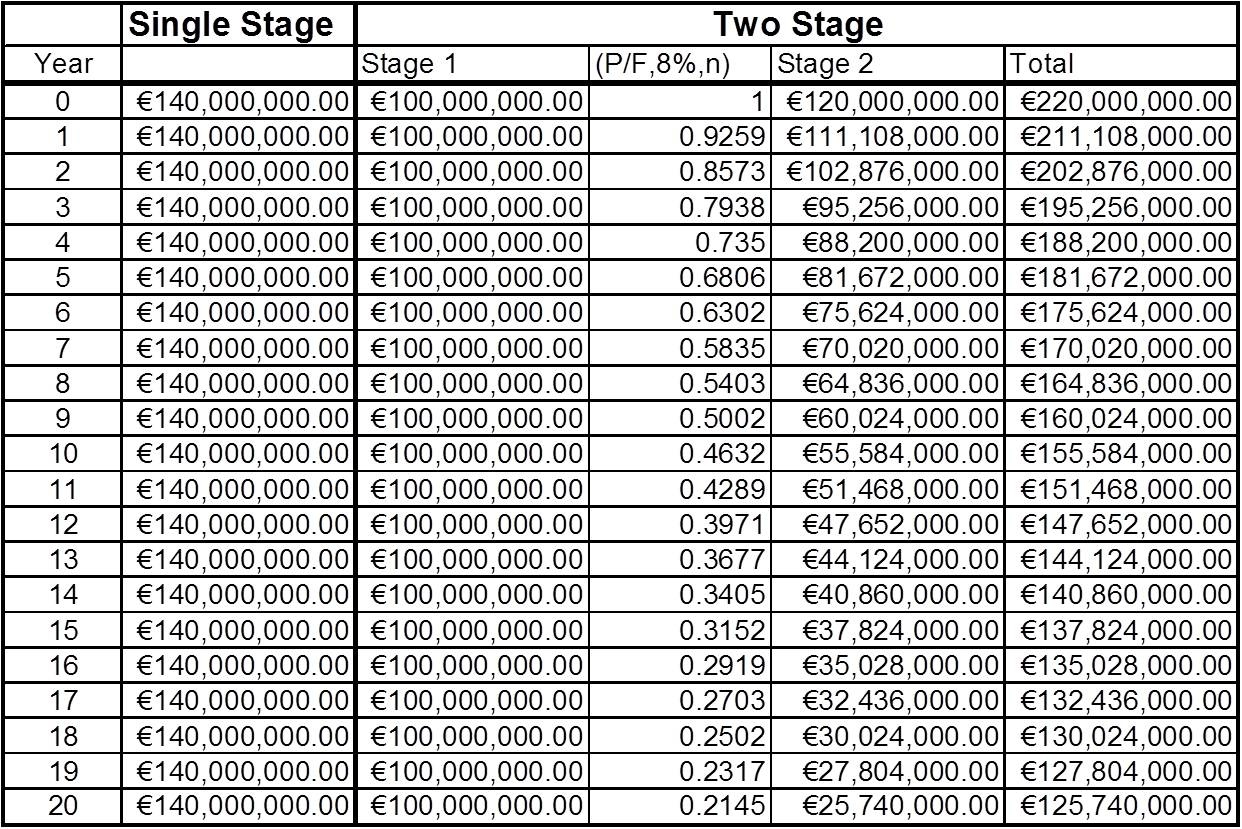
\includegraphics[width = 8cm]{images/table.jpg}
	\label{fig:sens1}
\end{figure}
\end{frame}\begin{center}\line(1,0){250}\end{center}





\begin{frame}
\frametitle{}
\begin{figure}
	\centering
		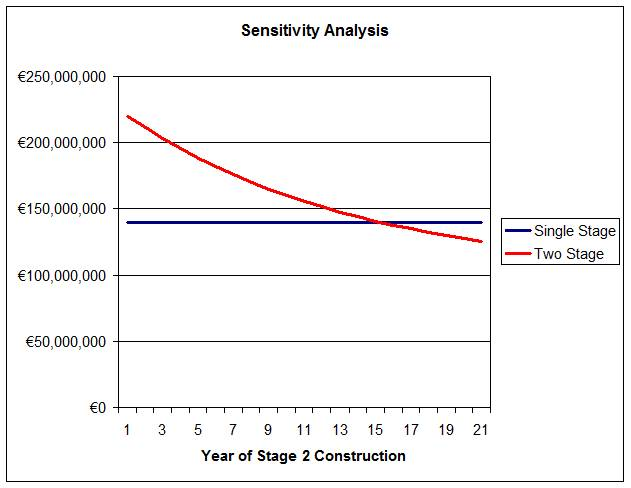
\includegraphics[width = 8cm]{images/sensgraph.jpg}
	\label{fig:sensgraph}
\end{figure}

After Year 15 it becomes more economical to build in two stages
\end{frame}\begin{center}\line(1,0){250}\end{center}





\begin{frame}
\frametitle{Quantitative Risk Analysis}
\begin{itemize}
\item Decision Tree
\begin{figure}
	\centering
		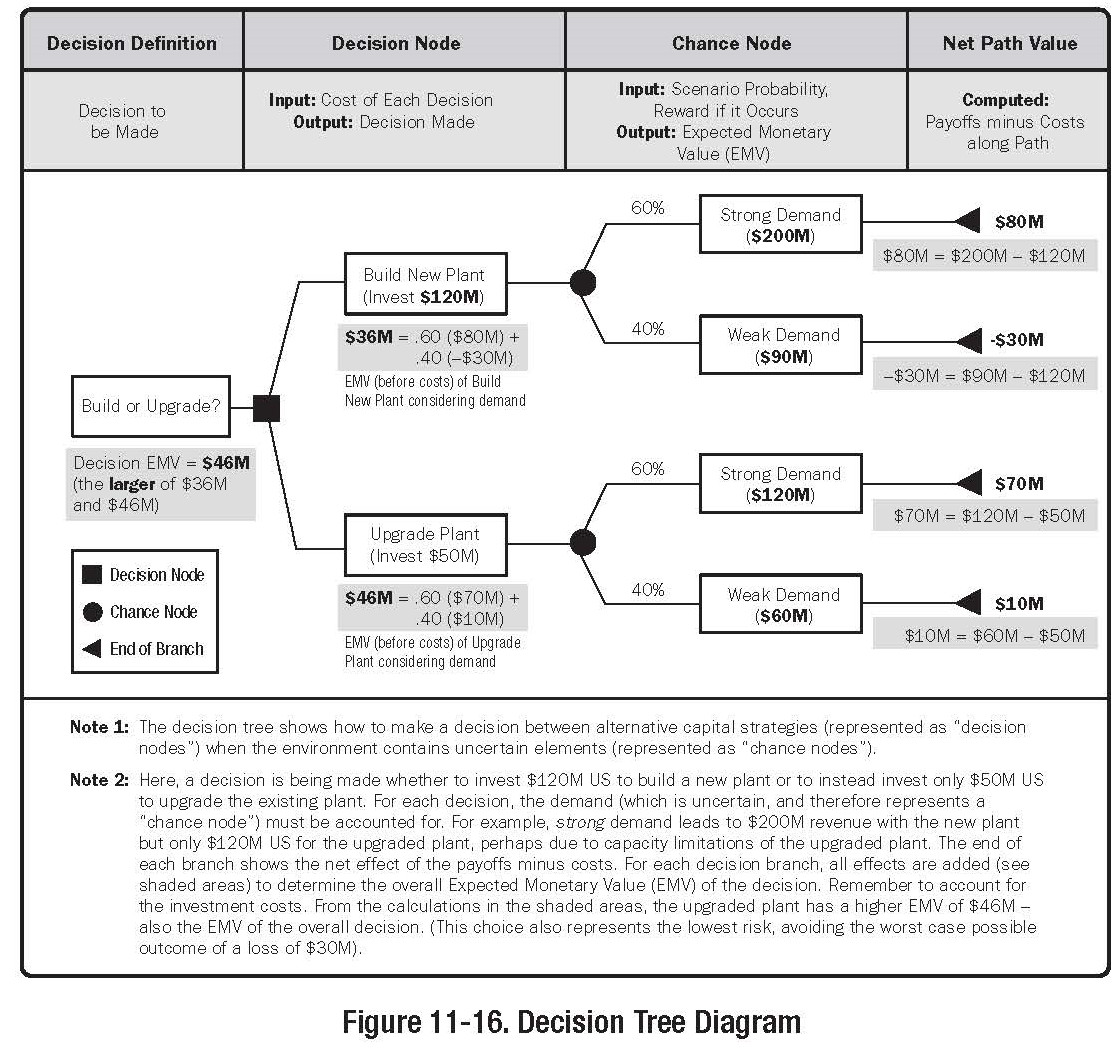
\includegraphics[width = 7cm]{images/Fig11-16.jpg}
	\label{fig:11-16}
\end{figure}
\end{itemize}
\end{frame}\begin{center}\line(1,0){250}\end{center}



\begin{frame}
\frametitle{Quantitative Risk Analysis}
\begin{itemize}
\item Modelling and Simulation (Monte Carlo)
\begin{figure}
	\centering
		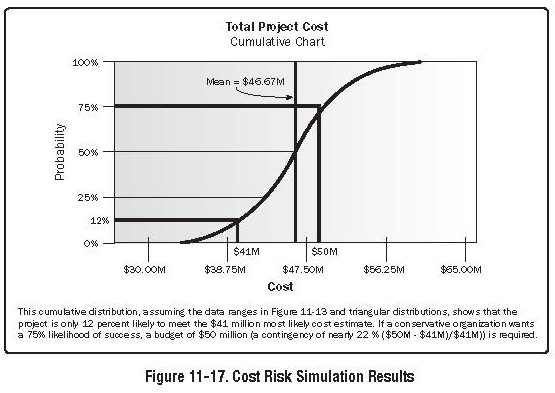
\includegraphics[width = 8cm]{images/Fig11-17.jpg}
	\label{fig:11-17}
\end{figure}
\end{itemize}
\end{frame}\begin{center}\line(1,0){250}\end{center}



\begin{frame}
\frametitle{Quantitative Risk Analysis}
\begin{itemize}
\item Outputs
\begin{itemize}
	\item Risk Register (Updates)
\end{itemize}
\item Probabilistic Analysis of the Project
\begin{itemize}
	\item Estimates of potential project schedule and cost outcomes
\item Usually expressed as a cumulative distribution 
� Fig. 11-13
\end{itemize}
\item Probability of achieving cost and time objectives
\begin{itemize}
	\item From fig 11-13, there is a 12% likelihood of achieving the cost estimate of $41M
\end{itemize}
\item Prioritised list of Quantified Risks
\begin{itemize}
	\item List of risks that pose the greatest threat, or the greatest opportunity to the project
\end{itemize}
\item Trends is Quantitative Risk Analysis Results
\begin{itemize}
	\item As analysis are repeated, trends may become apparent.
\end{itemize}
\end{itemize}
\end{frame}\begin{center}\line(1,0){250}\end{center}




\begin{frame}
\frametitle{Plan Risk Responses}
\begin{figure}
	\centering
		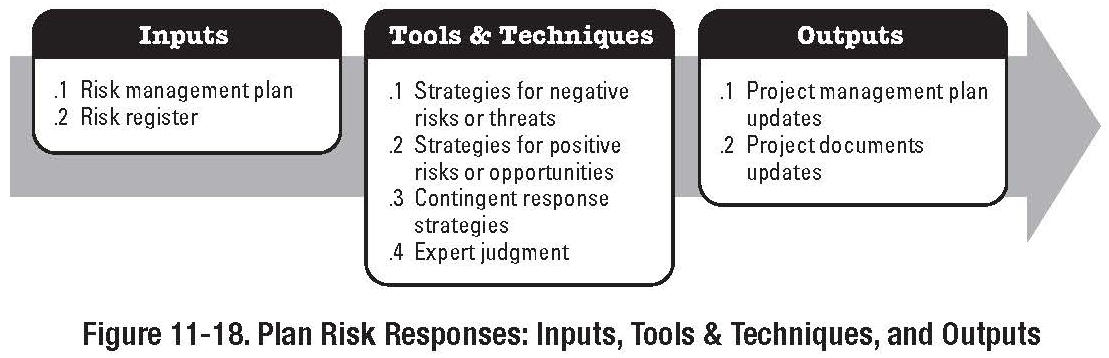
\includegraphics[width = 10cm]{images/Fig11-18.jpg}
	\label{fig:11-18}
\end{figure}
\begin{itemize}
\item Part of the Planning Process Group
\end{itemize}
\end{frame}\begin{center}\line(1,0){250}\end{center}






\begin{frame}
\frametitle{Plan Risk Responses}
\begin{itemize}
\item Risk Response Planning is the Process of developing options, and determining actions to enhance opportunities and reduce threats to the project's objectives.
\begin{itemize}
	\item Much of Risk Management focuses on negative risks; don't forget about opportunities
\end{itemize}
\item Risk Response Planning addresses risks by their priority by including resources, and activities into the budget, schedule, and PM plan, as needed.
\item Selecting the best response from several possible approaches is very common
\end{itemize}
\end{frame}\begin{center}\line(1,0){250}\end{center}





\begin{frame}
\frametitle{Plan Risk Responses}
\begin{itemize}
\item Inputs
\begin{itemize}
	\item Risk Management Plan
\end{itemize}
\item Roles and Responsibilities
\item Risk Analysis definitions, 
\item Risk Thresholds
\item Refer to book and previous notes
\begin{itemize}
	\item Risk Register
\end{itemize}
\item Defines root cause of risks
\item Includes potential responses, risk owners, symptoms, and warning signs
\item Includes Relative Rating of Risks
\end{itemize}
\end{frame}\begin{center}\line(1,0){250}\end{center}





\begin{frame}
\frametitle{Plan Risk Responses}
\begin{itemize}
\item Tools and Techniques
\begin{itemize}
	\item Strategies for Negative Risks or Threats
\end{itemize}
\item Avoid
\begin{itemize}
	\item Change PM Plan to eliminate risk or threat.
\item Isolate project objectives from risk's impact
\item Some risks can be avoided by clarifying requirements, obtaining information, improving communications, or acquiring expertise
\end{itemize}
\item Transfer
\begin{itemize}
	\item Shift negative impact of a threat, along with ownership of the response, to a third party (Insurance, Bonds, etc.)
\item Does not eliminate the risk; just transfers liability
\end{itemize}
\item Mitigate
\begin{itemize}
	\item Reduce the probability and/or impact to an acceptable level
\end{itemize}
� Process Improvement, Communications, Testing, Sign-off, etc.
\end{itemize}
\end{frame}\begin{center}\line(1,0){250}\end{center}



\begin{frame}
\frametitle{Plan Risk Responses}
\begin{itemize}
\item Tools and Techniques
\begin{itemize}
	\item Strategies for Positive Risks or Opportunities
\end{itemize}
\item Exploit
\begin{itemize}
	\item Measures to ensure positive risk is realised.
\end{itemize}
� Bonus-Penalty Clause in Contract
\item Share
\begin{itemize}
	\item Allocating ownership to a third party who is best able to capture the opportunity for the benefit of the project
\end{itemize}
� Joint Ventures..
\item Enhance
\begin{itemize}
	\item Maximisation of the opportunity or positive risk by identifying key drivers
\end{itemize}
� Lobbying for New Road to new/planned Industrial/Commercial Complex
\end{itemize}
\end{frame}\begin{center}\line(1,0){250}\end{center}




\begin{frame}
\frametitle{Plan Risk Responses}
\begin{itemize}
\item Strategy for Both Threats and Opportunities
\begin{itemize}
	\item Acceptance
\end{itemize}
\item Can be passive or active
\item Most common strategy for acceptance is the allocation of contingency reserves
\begin{itemize}
	\item Contingent Response Strategy
\end{itemize}
\item Responses designed to only come into operation or effect when predefined conditions occur
\item Trigger events: milestones, negative trends on CPI or SPI etc.
\end{itemize}
\end{frame}\begin{center}\line(1,0){250}\end{center}





\begin{frame}
\frametitle{Risk Response Planning}
\begin{figure}
	\centering
		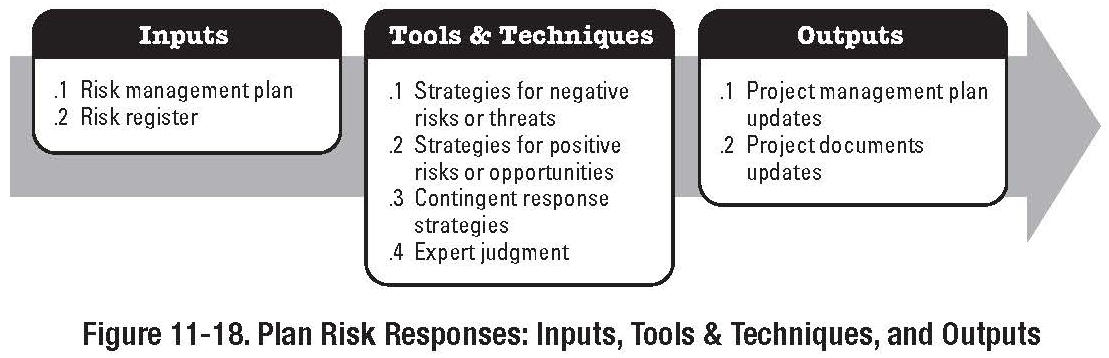
\includegraphics[width = 10cm]{images/Fig11-18.jpg}
	\label{fig:11-18}
\end{figure}
\begin{itemize}
\item Part of the Planning Process Group
\end{itemize}
\end{frame}\begin{center}\line(1,0){250}\end{center}



\begin{frame}
\frametitle{Risk Response Planning}
\begin{itemize}
\item Outputs
\begin{itemize}
	\item Risk Register Updates
\end{itemize}
\item After Risk Response Planning, the Risk Register needs to be updated to include the agreed Risk Responses
\begin{itemize}
	\item \item Refer to book for further details of Risk Register
\item Project Management Plan Updates
\end{itemize}
\item PM plan is likely to require changes via the Integrated Change Control Process in order to cater for changes in Budget, Schedule, Scope, etc., due to Risk Response Planning
\begin{itemize}
	\item Risk-Related Contractual Agreements
\end{itemize}
\end{itemize}
\end{frame}\begin{center}\line(1,0){250}\end{center}



\begin{frame}
\frametitle{Risk Response Planning}
\begin{itemize}
\item Outputs
\begin{itemize}
	\item Risk-Related Contractual Agreements
\end{itemize}
\item Such as Insurances, Bonds, Allocation etc.
\end{itemize}
\end{frame}\begin{center}\line(1,0){250}\end{center}




\begin{frame}
\frametitle{Risk Monitoring and Control}
\begin{figure}
	\centering
		\includegraphics[width = 10cm]{images/fig11-20.jpg}
	\label{fig:11-20}
\end{figure}
\begin{itemize}
\item Part of the Monitoring and Controlling Process Group
\end{itemize}
\end{frame}\begin{center}\line(1,0){250}\end{center}


\begin{frame}
\frametitle{Risk Monitoring and Control}
\begin{itemize}
\item Once Risk Responses are in place, it is still necessary to monitor and control risk throughout the project life-cycle.
\item Risk Monitoring and Control is the process of 
\begin{itemize}
	\item Identifying, and planning for newly arising risks 
\item Keeping track of identified risks and those on the watch-list
\item Reanalysing existing risks
\item Monitoring trigger conditions
\item Monitoring residual risks
\item Reviewing the execution of risk responses
\item Evaluating the effectiveness of risk responses 
\end{itemize}
\end{itemize}
\end{frame}\begin{center}\line(1,0){250}\end{center}


\begin{frame}
\frametitle{Risk Monitoring and Control}
\begin{itemize}
\item Other purposes of Risk Monitoring and Control are to determine if:
\begin{itemize}
	\item Project assumptions are still valid
\item Risk, as assessed, has changed from its prior state
\item Risk Management policies and procedures are being followed
\item Modifications are required to contingency reserves
\end{itemize}
\item New risks, unidentified risks, etc.
\end{itemize}
\end{frame}\begin{center}\line(1,0){250}\end{center}


\begin{frame}
\frametitle{Risk Monitoring and Control}
\begin{itemize}
\item Risk Monitoring and Control can involve
\begin{itemize}
	\item Choosing alternative strategies
\item Executing a contingency plan
\item Taking corrective action
\end{itemize}

\item Also includes
\begin{itemize}
	\item Updates to organisational process assets
\end{itemize}
\item Risk Database
\item Lessons Learned Data
\item Risk Management Templates
\end{itemize}
\end{frame}\begin{center}\line(1,0){250}\end{center}


\begin{frame}
\frametitle{Risk Monitoring and Control}
\begin{itemize}
\item Inputs
\begin{itemize}
	\item Risk Management Plan
\item Risk Register
\item Approved Change Requests
\end{itemize}
\item Can include changes to work methods, contract terms, scope and schedule
\begin{itemize}
	\item Work Performance Information
\end{itemize}
\item Deliverable Status; Corrective Actions; etc.
\begin{itemize}
	\item Performance Reports
\end{itemize}
\item Provide information on project work performance
\end{itemize}
\end{frame}\begin{center}\line(1,0){250}\end{center}



\begin{frame}
\frametitle{Risk Monitoring and Control}
\begin{itemize}
\item Tools and Techniques
\begin{itemize}
	\item Risk Reassessment
\end{itemize}
\item Identification of new risks, validation of previous risk assessments, etc.
\item Should be scheduled at regular intervals throughout the course of the project
\begin{itemize}
	\item Risk Audits
\end{itemize}
\item Examination and Documentation of the effectiveness of risk responses
\begin{itemize}
	\item Variance and Trend Analysis
\end{itemize}
\item Earned Value Management et al
\begin{itemize}
	\item Technical Performance Measurement
\end{itemize}
\item Actual Technical Performance against Baseline Plans
\begin{itemize}
	\item Reserve Analysis
\end{itemize}
\item Comparison of actual reserves against planned reserves throughout the project life-cycle to determine if remaining reserves are adequate  
\begin{itemize}
	\item Status Meetings
\end{itemize}
\end{itemize}
\end{frame}\begin{center}\line(1,0){250}\end{center}


\begin{frame}
\frametitle{Risk Monitoring and Control}
\begin{itemize}
\item Outputs
\begin{itemize}
	\item Risk Register Updates
\end{itemize}
 
\item Outcomes of risk assessments, risk audits and periodic risk reviews
\item Actual outcomes of project risks
\begin{itemize}
	\item Helps in determining risk probability; feeds into Risk Database etc.
\item Change Requests
\end{itemize}
\item Implementing Contingency Plans often involves changes to the overall Project Management Plan; these need to be run through the Integrated Change Control Procedures
\begin{itemize}
	\item Recommended Corrective Actions
\end{itemize}
\item Contingency Plans and Workarounds
\item Require Integrated Change Control
\end{itemize}
\end{frame}\begin{center}\line(1,0){250}\end{center}


\begin{frame}
\frametitle{Risk Monitoring and Control}
\begin{itemize}
\item Outputs
\begin{itemize}
	\item Recommended Preventative Actions
\end{itemize}
\item Recommendations to bring project back into compliance
\begin{itemize}
	\item Organisational Process Assets Updates
\end{itemize}
\item Risk Template Updates
\item Risk Database Updates
\begin{itemize}
	\item Project Document Updates
\end{itemize}
\end{itemize}
\end{frame}\begin{center}\line(1,0){250}\end{center}



\begin{frame}
\frametitle{Monte Carlo Simulation Example}
	A project is expected to cost \euro120,000.  Six independent risks and one opportunity have been identified during `Risk Identification'.
\begin{itemize}
\item A, cost of occurrence: \euro7,500; prob of occurrence 0.20  
\item B, cost of occurrence: \euro5,000; prob of occurrence 0.35 
\item C, cost of occurrence: \euro6,500; prob of occurrence 0.15 
\item D, cost of occurrence: \euro2,000; prob of occurrence 0.40 
\item E, cost of occurrence: \euro4,000; prob of occurrence 0.35
\item F, cost of occurrence: \euro2,500; prob of occurrence 0.10 
\item X, opportunity value: \euro3,500; prob of occurrence 0.12 
\end{itemize}
\end{frame}\begin{center}\line(1,0){250}\end{center}


\begin{frame}
\frametitle{Expected Monetary Value Example}
\begin{itemize}
\item Using simple Expected Monetary Value (EMV) analysis, the expected cost of the project is determined to be: 
\begin{figure}
	\centering
		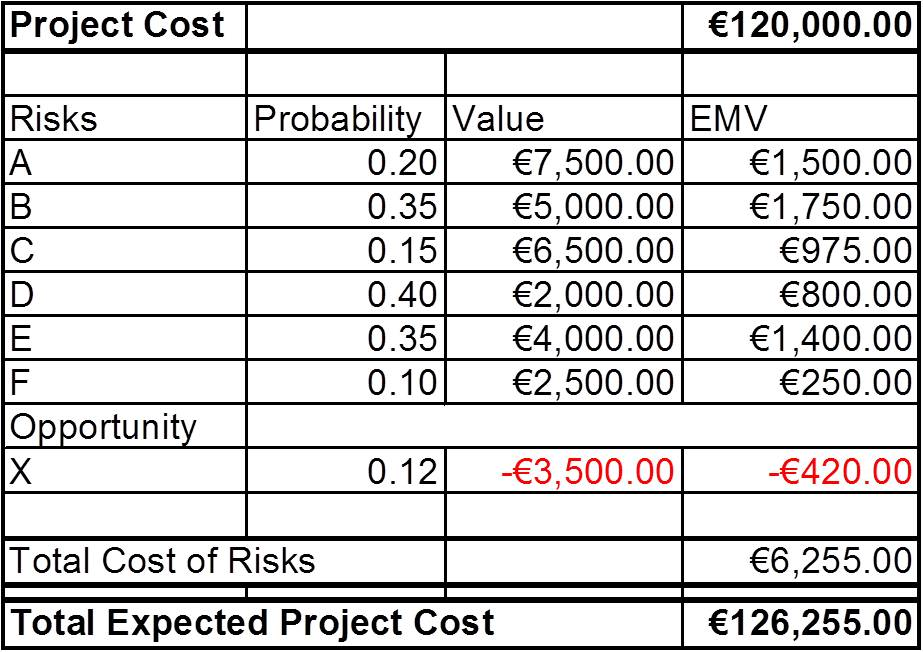
\includegraphics[width = 8cm]{images/evm1.jpg}
	\label{fig:evm}
\end{figure}
\end{itemize}
\end{frame}\begin{center}\line(1,0){250}\end{center}



\begin{frame}
\frametitle{Monte Carlo Simulation Example}
\begin{itemize}
\item Further simple analysis will yield
\begin{itemize}
	\item Max Project Cost: \euro147,500
\item Min Project Cost: \euro116,500
\item This yields a mean cost of \euro132,000
\end{itemize}
\end{itemize}
\end{frame}\begin{center}\line(1,0){250}\end{center}


\begin{frame}
\frametitle{Monte Carlo Simulation Example}
\begin{itemize}
\item You do not need to assign probabilities for a Monte Carlo Simulation
\begin{figure}
	\centering
		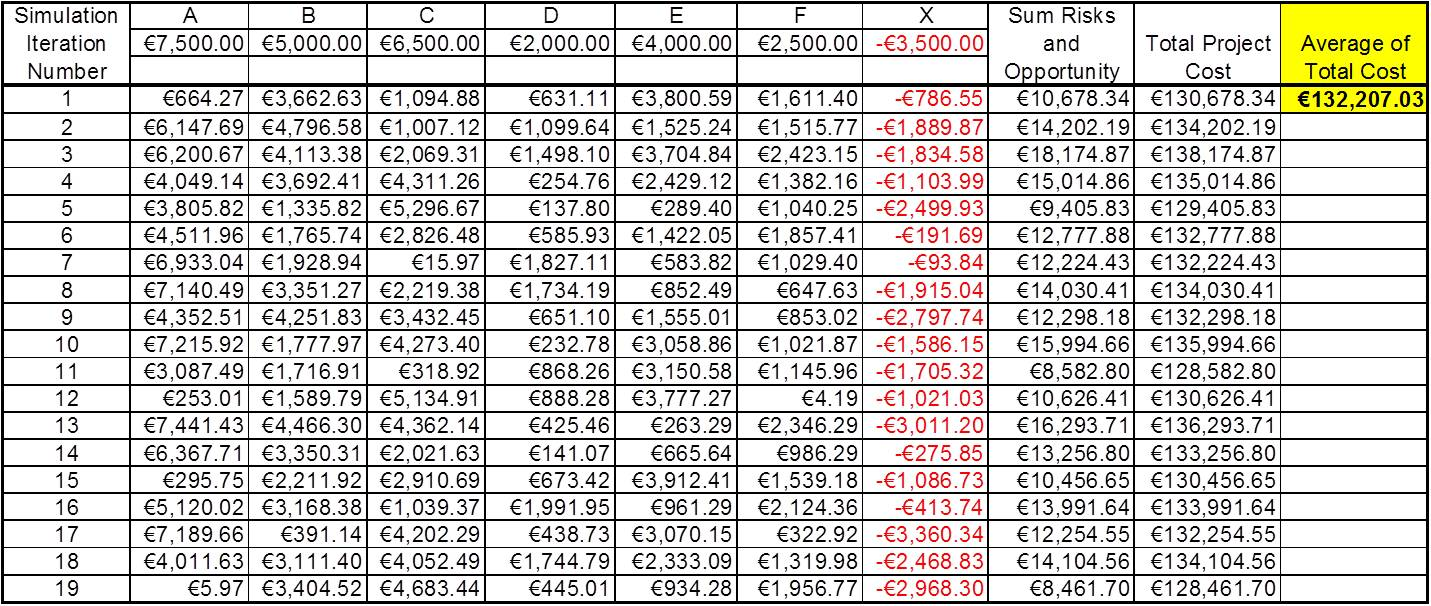
\includegraphics[width = 10cm]{images/montecarlo.jpg}
	\label{fig:mc1}
\end{figure}
\item The average figure ties in with the average determined by the max and min Project Costs
\end{itemize}
\end{frame}\begin{center}\line(1,0){250}\end{center}


\begin{frame}
\frametitle{Monte Carlo Simulation Example}
\begin{itemize}
\item So why undertake a Monte Carlo?
\begin{itemize}
	\item By undertaking an Monte Carlo simulation, additional information can be obtained, such as the standard deviation. (circa \euro3638.00)
\item Risks can also be modelled to more detail
\end{itemize}
\item For instance, If the cost of Risk Event a was a range as opposed to an exact figure, this aspect can also be modelled.
Range of A from \euro2,000 to \euro8,000; Yields Average of circa \euro130,000\begin{figure}
	\centering
		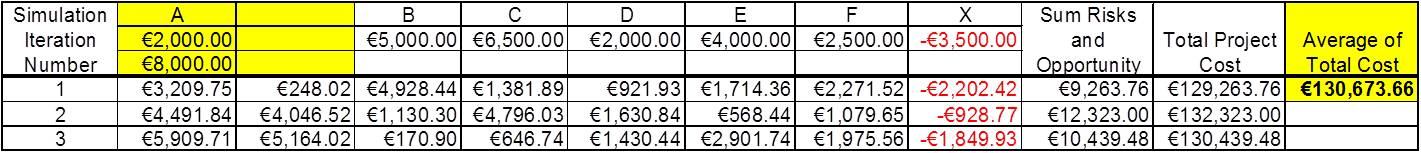
\includegraphics[width = 10cm]{images/montelimit.jpg}
	\label{fig:mc2}
\end{figure}
\end{itemize}
\end{frame}\begin{center}\line(1,0){250}\end{center}



\begin{frame}
\frametitle{Monte Carlo Simulation Example}
\begin{figure}[h]
	\centering
		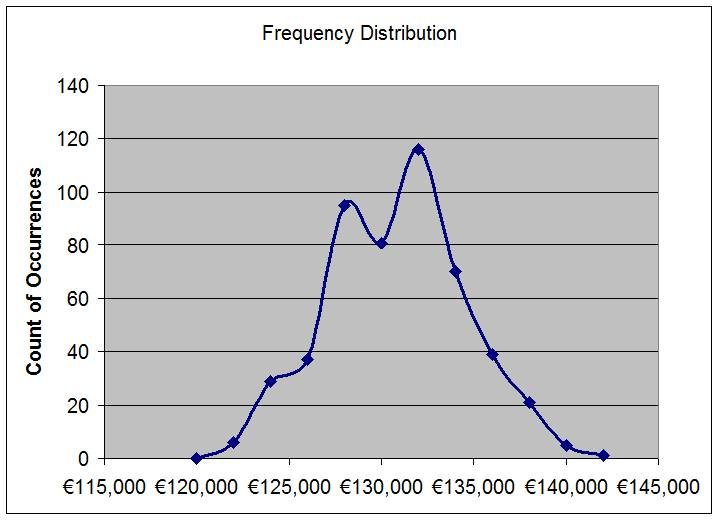
\includegraphics[width = 8cm]{images/montisample.jpg}
	\label{fig:montisample}
\end{figure}

\end{frame}\begin{center}\line(1,0){250}\end{center}







\begin{frame}
\frametitle{Monte Carlo Simulation Example}
\begin{figure}[h]
	\centering
		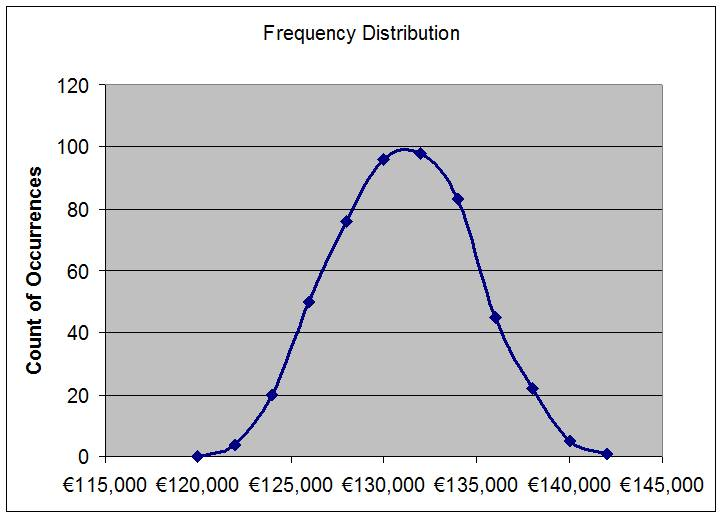
\includegraphics[width = 8cm]{images/montesample2.jpg}
	\label{fig:montesample2}
\end{figure}

\end{frame}\begin{center}\line(1,0){250}\end{center}

%% END OF LECTURE SLIDE
\begin{frame}
\frametitle{Next Lecture}{Reading:}
`A Guide to the Project Management Body of Knowledge'\\ 
Chapter 12 - Project Procurement Management
\begin{figure}[h]
	\centering
		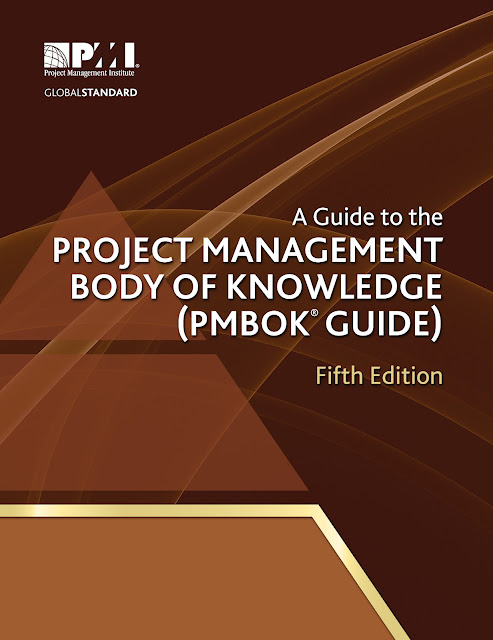
\includegraphics[width = 4cm]{images/book.jpg}
\end{figure}
\end{frame}\begin{center}\line(1,0){250}\end{center}
%% END OF LECTURE SLIDE



% End of slides
\end{document} 
